\documentclass[12pt]{article}

% Автор стиля: Сергей Копелиович
% Автор конспекта: Игорь Смирнов 

\usepackage{cmap}
\usepackage[T2A]{fontenc}
\usepackage[utf8]{inputenc}
\usepackage[russian]{babel}
\usepackage{graphicx}
\usepackage{amsthm,amsmath,amssymb}
\usepackage{listings}
\usepackage{color}
\usepackage{float}
\usepackage{xcolor}
\usepackage[normalem]{ulem}
\usepackage{array}
\usepackage{epigraph}

\usepackage[russian,colorlinks=true,urlcolor=red,linkcolor=blue]{hyperref}
\usepackage{enumerate}
\usepackage{datetime}
\usepackage{fancyhdr}
\usepackage{lastpage}
\usepackage{verbatim}
\usepackage{tikz}
\usetikzlibrary{arrows,decorations.markings,decorations.pathmorphing}
\usepackage{pgfplots}

\usepackage{ifthen}
\usepackage{mathtools}

%\usepackage{tabls}
%\usepackage{tabularx}
%\usepackage{xifthen}
%\listfiles

\def\SEASON{Технологии компьютерных сетей}

\input code-format.tex

\sloppy
\voffset=-20mm
\textheight=235mm
\hoffset=-22mm
\textwidth=180mm
\headsep=12pt
\footskip=20pt

\parskip=0em
\parindent=0em

\setlength\epigraphwidth{.8\textwidth}

\newlength{\tmplen}
\newlength{\tmpwidth}
\newcounter{listcounter}

% Список с маленькими отступами
\newenvironment{MyList}[1][4pt]{
  \begin{enumerate}[1.]
  \setlength{\parskip}{0pt}
  \setlength{\itemsep}{#1}
}{       
  \end{enumerate}
}
% Вложенный список с маленькими отступами
\newenvironment{InnerMyList}[1][0pt]{
  \vspace*{-0.5em}
  \begin{enumerate}[(a)]
  \setlength{\parskip}{-0pt}
  \setlength{\itemsep}{#1}
}{       
  \end{enumerate}
  \vspace*{-0.5em}
}
% Список с маленькими отступами
\newenvironment{MyItemize}[1][4pt]{
  \begin{itemize}
  \setlength{\parskip}{0pt}
  \setlength{\itemsep}{#1}
}{       
  \end{itemize}
}

% Основные математические символы
\def\TODO{{\color{red}\bf TODO}}
\def\N{\mathbb{N}}       %
\def\R{\mathbb{R}}       %
\def\F2{\mathbb{F}_2}    %
\def\Z{\mathbb{Z}}       %
\def\INF{\t{+}\infty}    % +inf
\def\EPS{\varepsilon}    %
\def\EMPTY{\varnothing}  %
\def\PHI{\varphi}        %
\def\SO{\Rightarrow}     % =>
\def\EQ{\Leftrightarrow} % <=>
\def\t{\texttt}          % mono font
\def\c#1{{\rm\sc{#1}}}   % font for classes NP, SAT, etc
\def\O{\mathcal{O}}      %
\def\NO{\t{\#}}          % #
\def\XOR{\text{ {\raisebox{-2pt}{\ensuremath{\Hat{}}}} }}
\renewcommand{\le}{\leqslant}
\renewcommand{\ge}{\geqslant}
\newcommand{\q}[1]{\langle #1 \rangle}               % <x>
\newcommand\URL[1]{{\footnotesize{\url{#1}}}}        %
% \newcommand{\sfrac}[2]{{\scriptscriptstyle\frac{#1}{#2}}}  % Очень маленькая дробь
% \newcommand{\mfrac}[2]{{\scriptstyle\frac{#1}{#2}}}    % Небольшая дробь
\newcommand{\sfrac}[2]{{\scriptstyle\frac{#1}{#2}}}  % Очень маленькая дробь
\newcommand{\mfrac}[2]{{\textstyle\frac{#1}{#2}}}    % Небольшая дробь

\newcommand{\fix}[1]{{\color{fixcolor}{#1}}} % \underline
\def\bonus{\t{\red{(*)}}}
\def\ifbonus#1{\ifthenelse{\equal{#1}{}}{}{\bonus}}
\def\smallsquare{$\scalebox{0.5}{$\square$}$}

\newlength{\myItemLength}
\setlength{\myItemLength}{0.3em}
\def\ItemSymbol{\smallsquare}
\def\Item{\vspace*{\myItemLength}\ItemSymbol \ \ }

\newcommand{\LET}{%
  % [line width=0.6pt]
  \begin{tikzpicture}%
  \draw(0.8ex,0) -- (0.8ex,1.6ex);%
  \draw(0,1.6ex) -- (0.8ex,1.6ex);%
  \end{tikzpicture}%
  \hspace*{0.1em}%
}

% Отступы
\def\makeparindent{\hspace*{\parindent}\unskip}
\def\up{\vspace*{-0.5em}}%{\vspace*{-\baselineskip}}
\def\down{\vspace*{0.5em}}
\def\LINE{\vspace*{-1em}\noindent \underline{\hbox to 1\textwidth{{ } \hfil{ } \hfil{ } }}}
\def\BOX#1{\mbox{\fbox{\bf{#1}}}}
\def\Pagebreak{\pagebreak\vspace*{-1.5em}}

% Мелкий заголовок
\newcommand{\THEE}[1]{
  \vspace*{0.5em}
  \noindent{\bf \underline{#1}}%\hspace{0.5em}
  \vspace*{0.2em}
}
% Другой тип мелкого заголовка
\newcommand{\THE}[1]{
  \vspace*{0.5em} $\bullet$
  \noindent{\bf #1}%\hspace{0.5em}
  \vspace*{0.2em}
}

\newenvironment{MyTabbing}{
  \t\bgroup
  \vspace*{-\baselineskip}
  \begin{tabbing}
    aaaa\=aaaa\=aaaa\=aaaa\=aaaa\=aaaa\kill
}{
  \end{tabbing}
  \t\egroup
}

% Код с правильными отступами
\lstnewenvironment{code}{
  \lstset{}
%  \vspace*{-0.2em}
}%
{
%  \vspace*{-0.2em}
}
\lstnewenvironment{codep}{
  \lstset{language=python}
}%
{
}

% Формулы с правильными отступами
\newenvironment{smallformula}{
 
  \vspace*{-0.8em}
}{
  \vspace*{-1.2em}
  
}
\newenvironment{formula}{
 
  \vspace*{-0.4em}
}{
  \vspace*{-0.6em}
  
}

% Большая квадратная скобка
\makeatletter
\newenvironment{sqcases}{%
  \matrix@check\sqcases\env@sqcases
}{%
  \endarray\right.%
}
\def\env@sqcases{%
  \let\@ifnextchar\new@ifnextchar
  \left\lbrack
  \def\arraystretch{1.2}%
  \array{@{}l@{\quad}l@{}}%
}
\makeatother

% Определяем основные секции: \begin{Lm}, \begin{Thm}, \begin{Def}, \begin{Rem}
\renewcommand{\qedsymbol}{$\blacksquare$}
\theoremstyle{definition} % жирный заголовок, плоский текст
\newtheorem{Thm}{\underline{Теорема}}[subsection] % нумерация будет "<номер subsection>.<номер теоремы>"
\newtheorem{Lm}[Thm]{\underline{Lm}} % Нумерация такая же, как и у теорем
\newtheorem{Ex}[Thm]{Упражнение} % Нумерация такая же, как и у теорем
\newtheorem{Example}[Thm]{Пример} % Нумерация такая же, как и у теорем
\newtheorem{Code}[Thm]{Код} % Нумерация такая же, как и у теорем
\theoremstyle{plain} % жирный заголовок, курсивный текст
\newtheorem{Def}[Thm]{Def} % Нумерация такая же, как и у теорем
\theoremstyle{remark} % курсивный заголовок, плоский текст
\newtheorem{Cons}[Thm]{Следствие} % Нумерация такая же, как и у теорем
\newtheorem{Conj}[Thm]{Гипотеза} % Нумерация такая же, как и у теорем
\newtheorem{Prop}[Thm]{Утверждение} % Нумерация такая же, как и у теорем
\newtheorem{Rem}[Thm]{Замечание} % Нумерация такая же, как и у теорем
\newtheorem{Remark}[Thm]{Замечание} % Нумерация такая же, как и у теорем
\newtheorem{Algo}[Thm]{Алгоритм} % Нумерация такая же, как и у теорем

% Определяем ЗАГОЛОВКИ
\def\SectionName{unknown}
\def\AuthorName{unknown}

\newlength{\sectionvskip}
\setlength{\sectionvskip}{0.5em}
\newcommand{\Section}[4][]{
  % Заголовок
  \pagebreak
%  \ifthenelse{\isempty{#1}}{
    \refstepcounter{section}
%  }{}
  \vspace{0.5em}
%  \ifthenelse{\isempty{#1}}{
%    \addtocontents{toc}{\protect\addvspace{-5pt}}%
    \addcontentsline{toc}{section}{\arabic{section}. #2}
%  }{}
  \begin{center}
    {\Large \bf Тема \NO{\arabic{section}}: #2} \\ 
    \vspace{\sectionvskip}
    {\large #3} \\
  \end{center}

  \LINE

  % Запомнили название и автора главы
  \gdef\SectionName{#2}
  \gdef\AuthorName{#4}

  % Заголовок страницы
  %\lhead{Алгоритмы, \SEASON}
  \chead{}
  \rhead{\SectionName}
  \renewcommand{\headrulewidth}{0.4pt}

  \lfoot{Глава \NO{\arabic{section}}. #3.}
  \cfoot{\thepage\t{/}\pageref*{LastPage}}
  \rfoot{Автор конспекта: \AuthorName}
  \renewcommand{\footrulewidth}{0.4pt}
}

\newcommand{\Subsection}[2][]{
  \refstepcounter{subsection}
  \vspace*{1em}
  \ifthenelse{\equal{#1}{}}
    {\addcontentsline{toc}{subsection}{\arabic{section}.\arabic{subsection}. #2}}
    {\addcontentsline{toc}{subsection}{\arabic{section}.\arabic{subsection}. \bonus\,#2}}
  {\color{blue}\bf\large \arabic{section}.\arabic{subsection}. \ifbonus{#1}\,{#2}} 
  \vspace*{0.5em}
  \makeparindent
}
\newcommand{\Subsubsection}[2][]{
  \refstepcounter{subsubsection}
  \vspace*{1em}
  \ifthenelse{\equal{#1}{}}
    {\addcontentsline{toc}{subsubsection}{\arabic{section}.\arabic{subsection}.\arabic{subsubsection}. #2}}
    {\addcontentsline{toc}{subsubsection}{\arabic{section}.\arabic{subsection}.\arabic{subsubsection}. \bonus\,#2}}
  {\color{blue}\bf\large \arabic{section}.\arabic{subsection}.\arabic{subsubsection}. \ifbonus{#1}\,#2}
  \vspace*{0.5em}
  \makeparindent
}

\newcommand{\Header}{
  \pagestyle{empty}
  \renewcommand{\dateseparator}{--}
  \begin{center}
    {\Large\bf 
     НИУ ВШЭ СПб, \SEASON\\
    \vspace{0.3em}
     По лекциям В.М. Ицыксона}\\
    \vspace{0.7em}
    {Собрано {\today} в {\currenttime}}
  \end{center}

  \LINE
  \vspace{0em}

  \renewcommand{\baselinestretch}{0.98}\normalsize
  \tableofcontents
  \renewcommand{\baselinestretch}{1.0}\normalsize
  \pagebreak
}

\newcommand{\BeginConspect}{
  \pagestyle{fancy}
  \setcounter{page}{1}
}

\definecolor{mygray}{rgb}{0.7,0.7,0.7}
\definecolor{ltgray}{rgb}{0.9,0.9,0.9}
\definecolor{fixcolor}{rgb}{0.7,0,0}
\definecolor{red2}{rgb}{0.7,0,0}
\definecolor{dkred}{rgb}{0.4,0,0}
\definecolor{dkblue}{rgb}{0,0,0.6}
\definecolor{dkgreen}{rgb}{0,0.6,0}
\definecolor{brown}{rgb}{0.5,0.5,0}

\newcommand{\green}[1]{{\color{green}{#1}}}
\newcommand{\black}[1]{{\color{black}{#1}}}
\newcommand{\red}[1]{{\color{red}{#1}}}
\newcommand{\dkred}[1]{{\color{dkred}{#1}}}
\newcommand{\blue}[1]{{\color{blue}{#1}}}
\newcommand{\dkgreen}[1]{{\color{dkgreen}{#1}}}

\begin{document}

\Header

\BeginConspect

\Section{Архитектуры компьютерных сетей}{Лекция 1}{Игорь Смирнов}

\Subsection{Эталонная модель ISO/OSI}

Компьютерные сети существуют давно (с 50-60 годов прошлого века), а потом появилось миллион протоколов и люди поняли, что невозможно связывать между собой различные системы. Тогда организация ISO создала стандарт OSI~--- эталонная модель взаимодействия открытых систем. Задачи поделены на 7 уровней. Для каждого уровня описаны функции и элементы данных, которыми компьютеры обмениваются на этом уровне.

\begin{figure}[H]
  \centering
  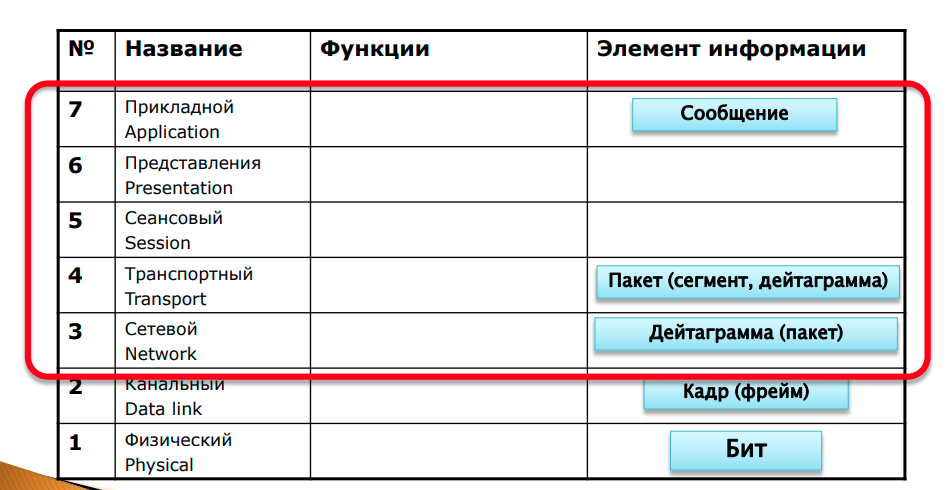
\includegraphics[width=15cm]{images/00/01}
\end{figure}

Иногда под физическим уровнем рисуют физическую среду, а над прикладным приложение/пользователя.

Эта стандартизация позволяет сравнивать между собой разные архитектуры и понимать, что за протокол используется и какая у него функциональная нагрузка.

\begin{enumerate}

\item Физический уровень позволяет соединить между собой два устройства и передать минимальную единицу информации~--- бит. Обычно объединён с канальным уровнем и говорят про протоколы канального-физического уровня.

\item Канальный объединяет между собой элементы компьютерной сети и позволяет двум узлам, находящимся в одной компьютерной сети обмениваться между собой потоками информации. Элемент информации~--- кадр (фрейм). Это последовательность бит, которая реализует канальный протокол. На канальном уровне могут обмениваться информацией только устройства, непосредственно соединённые канальной средой (проводной/оптической или беспроводной). То есть устройства видят друг друга без посредников. 

Примеры протоколов канального уровня: 
\begin{MyItemize}
    \item Ethernet (IEEE 802.3)
    \item Wi-Fi (IEEE 802.11)
\end{MyItemize}

\item Сетевой уровень предназначен для обмена информацией в многосегментной сети, где два конкретных узла могут быть не связаны между собой. Единица информации~--- дейтаграмма (пакет). Здесь реализуется функция адресации. Не обеспечивает никакой надёжности.

Примеры протоколов сетевого уровня:
\begin{MyItemize}
    \item IPv4
    \item IPv6
    \item ICMP
\end{MyItemize}

\item Транспортный уровень отвечает за транспортировку информации между приложениями. Раньше говорили про связь между узлами, а сейчас о конкретных приложениях. Здесь реализуется функция адресации приложений. Он обеспечивает определённый уровень надёжности транспортировки данных от одного приложения к другому. Элемент информации~--- пакет (иногда называют сегмент, иногда дейтаграмма).

Примеры протоколов транспортного уровня:
\begin{MyItemize}
    \item TCP
    \item UDP
\end{MyItemize}

\item Сеансовый уровень ко всему предыдущему добавляет возможность установления и разрыва логического канала между двумя участниками соединения. Специального названия у элемента информации нет. Если как-то и называют, то просто пакетом.

\item Уровень представления предназначен для согласования формата и кодировок информации с двух сторон. Например, общие алгоритмы сжатия информации, общие алгоритмы кодирования, представление в национальных языках. Обычно протоколов уровня исполнения в последнее время не бывает, а если и бывает, то элемент информации~--- пакет.

\item Прикладной уровень~--- реализация конкретных прикладных функций. Передача файла, передача электронной почты... Элемент информации~--- либо пакет, либо сообщение.

Примеры прикладных протоколов:
\begin{MyItemize}
    \item HTTP
    \item FTP
    \item ...
\end{MyItemize}

\end{enumerate}

Мы не будем заниматься 3-7 уровнями. 1 и 2 уровни реализуются аппаратно. 3-7~--- программно.

\Subsection{Архитектуры компьютерных сетей}

\begin{MyItemize}
    \item DNA (DECNet). В 80-90 годы была одной из доминирующих на рынке локальных и корпоративных компьютерных сетей. Проиграла TCP/IP
    \item SNA. Архитектура мейнфреймов в IBM. До сих пор используется в IBM. Имеет коннекты к TCP/IP. Широко не используется.
    \item DARPA (TCP/IP, Internet). Архитектура американского министерства обороны. 
    \item Novell Netware. Раньше была монополистом в области локальных сетей. Тоже проиграла TCP/IP
    \item SMB. Частично используется в сервисах верхнего (транспортный и выше) уровня. В Microsoft и IBM используется для общего доступа к ресурсам
    \item AppleTalk. <<Сейчас имеет историческое значение>>
    \item XNS (читается зи эн эс). От компании Xerox
    \item IPv6. Ответвление от DARPA. Прекрасный интернет будущего
\end{MyItemize}

Изучать будем DARPA и IPv6. 

\Subsection{Характеристики архитектур компьютерных сетей}

\begin{enumerate}
    \item Иерархия протоколов. Показывает то, как архитектура устроена, как протоколы взаимодействуют между собой
    \item Соответствие модели ISO. 
    \item Адресация
    \begin{enumerate}
        \item Узлов
        \begin{enumerate}
            \item Индивидуальная (один адрес $\leftrightarrow$ 1 компьютер/сетевой интерфейс)
            \item Групповая (один адрес $\rightarrow$ несколько узлов)
            \item Широковещательная (один адрес $\rightarrow$ все адреса какого-то подмножества сети)
        \end{enumerate}
        В IPv4 есть все три, в IPv6 широковещательная реализована через групповую
        \item Приложений
    \end{enumerate}
    \item Связь с канальным уровнем. Нужно оборачивать пакеты сетевой среды в кадры канальной среды. Для этого есть разные механизмы.
    \begin{enumerate}
        \item Разрешение адресов (мапа адресов сетевого уровня на адреса канального уровня). Протокол, позволяющий запрашивать MAC адрес и прочее~--- это как раз про это
        \item Фрагментация. В сетевом и канальном уровне есть ограничения на размеры пакета/кадра. Эти ограничения бывают разными. Поэтому иногда надо большие пакеты сетевого нарезать в маленькие кадры канального.
        \begin{enumerate}
            \item Поузловая. Каждый узел, получив пакет, сам занимается фрагментацией
            \item На источнике. С самого начала делим на маленькие кусочки
        \end{enumerate}
        В IPv4 используется поузловая. А в IPv6 на источнике.  
    \end{enumerate}
    \item Сетевые протоколы. Основа любой архитектуры
    \item Маршрутизация. Доставка пакета через сложную сеть от одного узла к другому
    \begin{enumerate}
        \item По типу маршрута
        \begin{enumerate}
            \item Индивидуальная (когда доставляем одному узлу)
            \item Групповая (когда доставляем группе)
        \end{enumerate}
        В IPv4 и то, и то
        \item По адаптивности изменения в сети
        \begin{enumerate}
            \item Статическая (каждый маршрутизатор знает что делать с каждым пакетом)
            \item Динамическая (на лету решаем, что делать с пакетом)
            \item Предопределённая (<<от источника>>) (весь маршрут пакета задаётся на источнике)
        \end{enumerate}
        В IPv4 и IPv6 статическа и динамическая. Для тестирования можно и предопределённую.
        \item По месту проведения маршрутных вычислений
        \begin{enumerate}
            \item Централизованная (есть один узел, который принимает решения о том, как доставлять, по всем маршуртам)
            \item Децентрализованная (каждый решает сам)
            \item Гибридная
        \end{enumerate}
        В сетях TCP/IP децентрализованная и гибридная. Централизованная используется в неком <<ныне популярном>> SDN
        \item По числу возможных маршрутов
        \begin{enumerate}
            \item Однопутевые (на одну сеть сохраняется один маршрут)
            \item Многопутевые (на одну сеть несколько маршрутов)
        \end{enumerate}
        В TCP/IP в основном однопутевые, но есть несколько многопутевых протоколов.
        \item По характеру используемой информации для принятия решения
        \begin{enumerate}
            \item Глобальные (нужно знать топологию всей сети)
            \item Локальные (знаем информацию о соседях)
            \item Смешанные (знаем о соседях и ещё о какой-то части сети)
        \end{enumerate}
        В TCP/IP локальные и смешанные
    \end{enumerate}
    \item Транспортные механизмы
    \begin{enumerate}
        \item Дейтаграммные. Транспортировка путём посылки дейтаграмм без гарантии поставки и времени порядка их прихода
        \item Потоковые. Гарантия доставки, сохранение последовательности передачи пакетов
        \item Многопоточные. Между приложениями несколько потоков. Внутри каждого потока гарантии как у потокового
    \end{enumerate}
    В TCP/IP дейтаграммный это UDP, потоковый~--- TCP. Есть SCTP. Не получил широкого распространения, но это многопоточный и входит в TCP/IP
    \item Именование ресурсов
    \item По типу маршрута. Мнемонические имена, которые используются, чтобы людям было удобнее работать
    \begin{enumerate}
        \item Одноуровневое
        \item Двухуровневое
        \item Иерархическое
    \end{enumerate}   
    В TCP/IP иерархическая (spb.hse.ru)
    \item Прикладные протоколы
    \begin{enumerate}
        \item Удалённый терминал
        \item Передача файлов
        \item Электронная почта
        \item ...
    \end{enumerate}
    \item Управление
    \item Защита информации
\end{enumerate}

Изучив эти 11 характеристик, можно понять, как работает архитектура. Мы будем изучать всё это про DARPA.

\Subsection{История создания}

В 1957 создали организацию DARPA при министерстве обороны.

В 1968 там создали сеть ARPANET.

В 1969 впервые передали данные между двумя университетами. По легенде, один послал другому 1 байт, после чего оба зависли.

В 1974 разработали TCP/IP. 

В 1983 ARPANET перешёл с NCP на TCP/IP.

В 1984 создали DNS.

1989~--- создание WWW и первой версии HTTP.

В 1990 приняли единый термин Internet (вместо ARPANET).

1993~--- первый браузер Mosaic.


\begin{figure}[H]
  \centering
  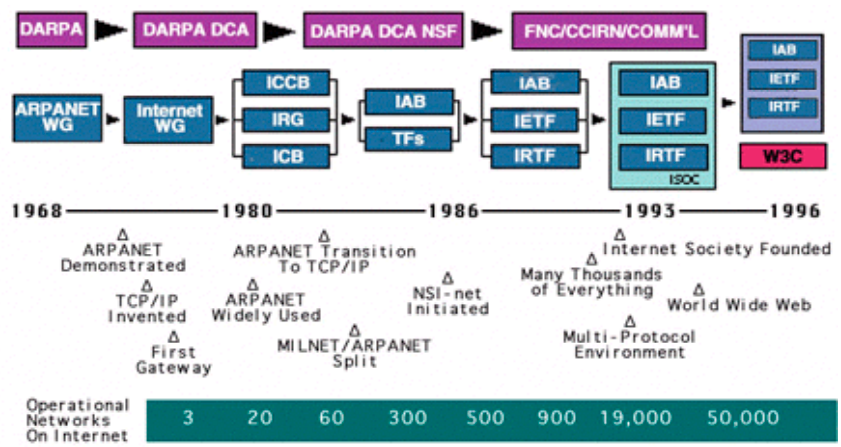
\includegraphics[width=15cm]{images/00/02}
\end{figure}

\Subsection{Стандартизирующие организации Internet}


Internet Society (ISOC)~--- сообщество, занимающееся развитием Internet
\begin{enumerate}
    \item Internet Architecture Board (IAB)~--- координирует развитие TCP/IP
    \begin{enumerate}
        \item Internet Engineering Steering Group (IESG)~--- рассмотрение стандартов и технические работы для IETF
        \item Internet Engineering Task Force (IETF)~--- самый главный комитет. Выпускают RFC
        \item Internet Research Task Force (IRTF)~--- развитие технологий, которые могут понадобиться в будущем
        \item Internet Corporation for Assigned Names and Numbers (ICANN)~--- централизованное назначение адресов и номеров (ранее IANA)
    \end{enumerate}
\end{enumerate}

\Subsection{Координирующие организации Internet}

Network Information Center (NIC)~--- организации, ответственные за распределение адресов
\begin{enumerate}
    \item InterNIC~--- США
    \item Reseaux IP Europeens (RIPE)~--- Европа
    \item African Network Information Centre (AfriNIC)~--- Африка
    \item Asia Pacific Network Information Centre (APNIC)~--- Азия
    \item Regional Latin-American and Caribbean IP Address Registry (LACNIC)~--- Латинская Америка
    \item Russian Institute for Public Networks (RIPN)~--- Россия
\end{enumerate}

\Subsection{Стандарты TCP/IP}

Все стандарты TCP/IP~--- это текстовые документы с уникальным номером (RFC). Все они лежат на ietf.org/rfc.html

Там нет жёсткой стандартизации, некоторые места можно истолковать двояко, не все им следуют.

Сначала их делили на FYI и STD. В последнее время так не делают

\Subsection{Иерархия протоколов TCP/IP}

\begin{figure}[H]
  \centering
  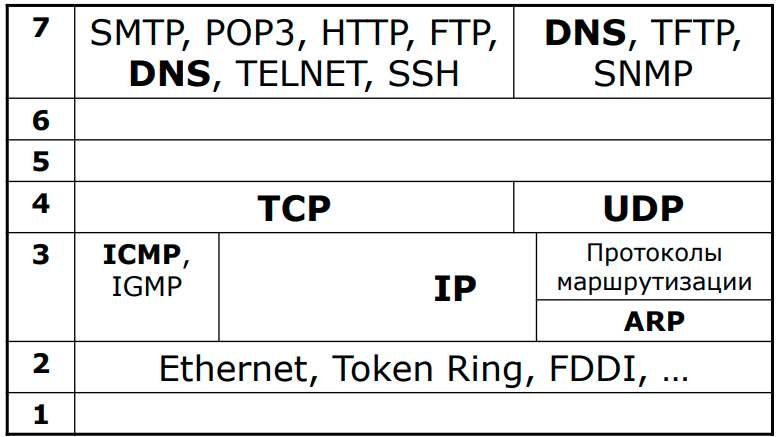
\includegraphics[width=15cm]{images/00/03}
\end{figure}

Самым важным протоколом является протокол сетевого уровня IP. На сетевом уровне находятся также ICMP (протокол управляющих сообщений, расширяет собой IP) и IGMP (протокол групповых сообщений), ARP (связь с канальным уровнем), огромное число протоколов маршрутизации.

На транспортном уровне TCP и UDP. 

На сеансовом уровне и уровне представления протоколов нет, поскольку кусок роли установления сеанса выполняет TCP (в UDP сеанса вообще нет). В TCP/IP шестого уровня нет. То есть каждый раз реализуем представительский протокол. Это жутко неудобно, привело к куче проблем и это архитектурная ошибка.

На прикладном уровне миллион разных протоколов. Слева транспорт TCP, справа~--- UDP. 


\Section{Адресация в IP}{Лекции 1-2}{Игорь Смирнов}

IP-адрес: 32 разряда

Записывается в виде десятичных октетов, разделённых точкой.

Можно адресовать $2^{32}$ узлов ($\approx 4\text{ млрд.}$)

Но не все из них поддерживаются.

Поддерживаются индивидуальная, групповая и широковещательная адресации.

Адресуется конкретный сетевой интерфейс, а не узел. Поэтому если у компьютера  сетевых интерфейса, то у него должно быть $\ge 3$ сетевых адреса. Некорректно говорить про IP-адрес узла.

И одному интерфейсу может соответствовать несколько IP-адресов. Например, если один интерфейс находится сразу в нескольких сетях.

Иногда (очень редко) можно дать один адрес нескольким интерфейсам.

Адресное пространство поделено на классы:

\begin{enumerate}
    \item Класс A~--- сети большого размера
    \item Класс B~--- сети среднего размера
    \item Класс C~--- небольшие сети
    \item Класс D~--- групповые адреса
    \item Класс E~--- для эКсПеРиМеНтОв
\end{enumerate}

Как это всё было изначально:

\Subsubsection{Адреса класса A}

Формат адреса: {\tt 0nnnnnnn.hhhhhhhh.hhhhhhhh.hhhhhhhh}

$n$~--- номер сети
$h$~--- номер узла

То есть можно сделать 128 сетей (а на самом деле 126, потому что 2 зарезервированы) по $2^{24}-2$ узлов в каждой.

Таким образом, все адреса в диапазоне {\tt 1.0.0.0-126.255.255.255}. Даже сейчас столько адресов ни одной компании не нужно. Поэтому их используют по-другому. Как именно~--- узнаем позже.

\Subsubsection{Адреса класса B}

Формат адреса: {\tt 10nnnnnn.nnnnnnnn.hhhhhhhh.hhhhhhhh}

{\tt n}~--- номер сети
{\tt h}~--- номер узла

$2^{14}$ сетей (тут уже нет двух зарезервированных), по $2^{16}-2$ узлов в каждой.

Диапазон адресов {\tt 128.0.0.0-191.255.255.255}

Это очень большие сети, таких размеров хватает крупнейшим корпорациям.

\Subsubsection{Адреса класса C}

Формат адреса: {\tt 110nnnnn.nnnnnnnn.nnnnnnnn.hhhhhhhh}

{\tt n}~--- номер сети
{\tt h}~--- номер узла

$2^{21}$ сетей, по 254 узла.

Диапазон адресов {\tt 192.0.0.0-223.255.255.255}

\Subsubsection{Адреса класса D}

Групповые адреса Internet.

Формат адреса: {\tt 1110xxxx.xxxxxxxx.xxxxxxxx.xxxxxxxx}

$2^{28}$ адресов, диапазон: {\tt 224.0.0.0 - 239.255.255.255}

Пример использования: вещание радиостанции на групповом адресе. Поднимаем на компьютере соответствующий IP-адрес. Тогда автоматически будет приходить нужный трафик.

К сожалению, используется редко (хотя зря).

\Subsubsection{Адреса класса E}

Зарезервированы для экспериментов

Формат адреса: {\tt 1111xxxx.xxxxxxxx.xxxxxxxx.xxxxxxxx}

$2^{28}$ адресов

Диапазон: {\tt 240.0.0.0-254.255.255.255}

Никогда пакет, приходящий из интернета не должен иметь класс E. Такие надо фильтровать.

\Subsection{Зарезервированные адреса}

\begin{MyItemize}
    \item Адрес {\tt 0.0.0.0}

    Если встречаете его в таблице маршрутизации, то это <<маршрут по умолчанию>>. Если встречаете его при адресации, то это <<данная сеть>>. Второе никогда не используется.
    \item Узел данной сети

    Вместо адреса сети записываем нули.

    A: {\tt 00000000.hhhhhhhh.hhhhhhhh.hhhhhhhh}\\
    B: {\tt 10000000.00000000.hhhhhhhh.hhhhhhhh}\\
    C: {\tt 11000000.00000000.00000000.hhhhhhhh}

    Но по факту это практически нигде не реализовано.

    \item Конкретная IP-сеть ($^*$)

    Вместо адреса узла~--- нули.

    A: {\tt 0nnnnnnn.00000000.00000000.00000000}\\
    B: {\tt 10nnnnnn.nnnnnnnn.00000000.00000000}\\
    C: {\tt 110nnnnn.nnnnnnnn.nnnnnnnn.00000000}

    Адресуем целую сеть. Используется в таблицах маршрутизации, когда хотим указать одинаковый маршрут для всей сети.

    \item Все узлы данной IP-сети ($^*$)

    Вместо адреса узла~--- единицы.

    A: {\tt 0nnnnnnn.11111111.11111111.11111111}\\
    B: {\tt 10nnnnnn.nnnnnnnn.11111111.11111111}\\
    C: {\tt 110nnnnn.nnnnnnnn.nnnnnnnn.11111111}

    Широковещательный адрес. Пакет придёт ко всем узлам этой сети. 

    Но по факту для сетей класса A и класса B не используется, потому что это мечта хакера. Посылаем 1 пакет, а его получают миллионы пользователей.

    Иногда блокируется вообще весь широковещательный трафик.

\end{MyItemize}

По сути последние два~--- это одно и то же. Только первое используется в таблицах маршрутизации, а второе в конкретных IP-пакетах, поэтому теоретически могли бы использовать только один из них, но почему-то так не сделали.

Из-за последних двух мы делали минус два, когда считали количество узлов в сети.

\begin{MyItemize}
    \item Все узлы данной локальной сети: {\tt 255.255.255.255}.

    Это отличается от <<Все узлы сети>> тем, что тут мы адресуем только те узлы, что подключены к нам канальным способом. То есть это широковещательный канальный адрес. В предыдущем же~--- сетевой уровень. Предыдущий маршрутизируется, а этот нет.

    \item Петля обратной связи.

    {\tt 01111111.xxxxxxxx.xxxxxxxx.xxxxxxxx}

    {\tt 127.0.0.1}~--- принято использовать.

    Не имеет внешнего выхода. Это обращение к самому себе через весь сетевой стек. 

    127~--- это сеть класса A. Нулевой и 127 занят, поэтому сетей класса A 126.
\end{MyItemize}

Так было в начале. Но потом добавили ещё несколько зарезервированных адресов.

IANA зарезервировала для внутреннего использования адреса <<неанонсированной сети>>. Когда разворачиваем локальную сеть и у нас нет полученных легальным образом адресов, мы можем использовать сеть из RFC1918:

\begin{MyItemize}
    \item {\tt 10.0.0.0-10.255.255.255}
    \item {\tt 172.16.0.0-172.31.255.255}
    \item {\tt 192.168.0.0-192.168.255.255}
\end{MyItemize}

Что будет если поставим себе другой адрес? Допустим, если мы поставили себе адрес майкрософта, мы отрежем себе доступ ко всему майкрософту.

А ещё есть зарезервированные адреса в сетях класса D.

\begin{MyItemize}
    \item {\tt 224.0.0.1}~--- все узлы данной подсети
    \item {\tt 224.0.0.2}~--- все маршрутизаторы данной подсети
    \item {\tt 224.0.0.5}~--- все OSPF маршрутизаторы
    \item {\tt 224.0.0.6}~--- все назначенные OSPF маршрутизаторы
    \item {\tt 224.0.0.9}~--- все RIP-2 маршрутизаторы
    \item {\tt 224.0.0.10}~--- все IGRP маршрутизаторы
\end{MyItemize}

\Subsection{Структуризация сетей IP}

В том, что мы обсуждали ранее много недостатков. Например, то, что много адресов вообще не используются. Поэтому придумали структуризацию сетей IP.

Теперь мы будем по-другому интерпретировать разряды адреса. Если раньше у нас были {\tt n} и {\tt h}, то теперь будет {\tt n}, {\tt s}, {\tt h}. {\tt s}~--- подсеть.

Маска подсети~--- это 32-х разрядный вектор флагов. Если в $i$-ом разряде маски стоит 1, то $i$-й разряд адреса содержит часть номера сети/подсети, а если 0, то часть номера узла.

Таким образом, с помощью адреса и маски, можно более гибко разделить сеть, чем с помощью адреса и класса.

Например, сеть класса C можем разделить на 2 подсети по 128 адресов с помощью маски {\tt 255.255.255.128}, на 4 подсети по 64 адреса с помощью маски {\tt 255.255.255.192}, 8 подсетей по 32 адреса с маской {\tt 255.255.255.224} ну и так далее.

Но вот 128 подсетей по 2 адреса~--- не работает. Потому что первый и последний адрес у нас зарезервированы. Поэтому минимальная подсеть содержит 4 адреса, 2 из которых зарезервированы.

Аналогично на подсети можно делить сети классов A и B.

В одной сети можно иметь подсети разного размера (стандарт VLSM).

Но у подсетей есть проблема (с первой и последней), потому что там есть широковещательные адреса (все нолики и все единички) и непонятно, к чему их применять (ко всей сети или к подсети). Поэтому сначала вообще не использовали первую и последнюю подсети. Однако потом подумали и поняли, что такая коллизия почти никогда не встречается, потому что всегда с нулевым адресом идёт маска, а широковещательную адресацию никто не использует. В итоге почти все маршрутизаторы позволяют использовать первую и последнюю подсети.

Принято, что сначала в маске идут разряды сети/подсети, а потом~--- узла (то есть префикс из единиц, а потом все нули). То есть теперь масок может быть всего 31 (маски из всех единиц быть не может, маска с одним ноликом бессмысленна). Кстати, маска с одной единицей тоже бессмысленна.

{\bf Префикс сети}~--- число единиц в маске (полагаем, что маска удовлетворяет предыдущему требованию).

Например, для маски {\tt 255.255.255.240} префикс сети~--- 28.

Подсеть записывается так: {\tt 195.19.212.96/27}, то есть IP-адрес первого узла, слеш и префикс. Этот адрес соответствует подсети {\tt 195.19.212.96-195.19.212.127}

Для стандартных сетей префиксы такие:
\begin{MyItemize}
    \item A~--- 8
    \item B~--- 16
    \item C~--- 24
\end{MyItemize}

\Subsubsection{Надсети}

Обратная идея: хотим объединять несколько соседних сетей.

Например, хотим объединить {\tt 195.19.212.0} и {\tt 195.19.213.0}

Объединим в надсеть {\tt 195.19.212.0/255.255.254.0} (префикс 23).

А теперь хотим объединить {\tt 192.168.1.0} и {\tt 192.168.2.0}.

Тут так не получится. Можем объединить только в сеть на 1024 адреса с префиксом 22: {\tt 192.168.0.0/255.255.252.0}

\Subsubsection{Задачки}

A~--- IP-адрес узла\\
M~--- маска подсети

Адрес подсети: {\tt Net = A\&M}\\
Широковещательный адрес: {\tt Broad=A|(!M)}\\
Размер подсети: {\tt K = (!M) - 1} (минус 1, потому что первый и последний адрес зарезервированы)

\Subsection{Адресация сервисов (приложений)}

{\bf Порт}~--- уникальный номер приложения на узле, использующего конкретный транспортный протокол.

В TCP/IP порт~--- это число от 0 до 65535.

Приложение в сети идентифицируется сокетом. {\bf Сокет}~--- это IP-адрес узла, тип транспортного протокола и номер порта.

Примеры:
\begin{MyItemize}
    \item TCP-сокет: {\tt 195.19.212.13:80}
    \item UDP-сокет: {\tt 195.19.212.10:53}
\end{MyItemize}

По соглашению, диапазон портов от 0 до 1023 зарезервирован за well-known серверными службами. Остальные, непривилегированные порты, могут использоваться любыми приложениями. 

\Section{Сетевой уровень TCP/IP}{Лекция 2}{Игорь Смирнов}

Протоколы:
\begin{itemize}
    \item IP~--- основной протокол архитектуры TCP/IP
    \item ICMP~--- протокол управляющих сообщений
    \item IGMP~--- протокол работы с группами
    \item ARP~--- протокол разрешения адресов~--- связь между собой адресов канального и сетевого уровней
    \item Протоколы маршрутизации
\end{itemize}

\Subsection{Протокол IP}

{\bf IP}~--- Internet Protocol

Стандарт RFC 791, 1981 год

Текущая действующая версия~--- 4 (IPv4)

Состоит из заголовка и тела

Суммарная длина до 64 Кбайт

Структура IP-пакета:

TODO: картинка

Ширина картинки~--- 32 разряда. Под каждым полем подписано, сколько разрядов оно занимает.

\begin{itemize}
    \item V~--- версия протокола
    \item HL~--- длина заголовка в 32-разрядных словах
    \item TOS~--- пожелания к процедуре обслуживания данного пакета
    \item Length~--- длина пакета в байтах
    \item ID~--- идентификатор (для фрагментации)
    \item F~--- флаги (для фрагментации)
    \item Offset~--- смещение (для фрагментации)
    \item TTL~--- время жизни
    \item Protocol~--- вложенный протокол (в данных)
    \item HCRC~--- контрольная сумма (по заголовку)
    \item Source Address~--- адрес отправителя
    \item Destination Address~--- адрес получателя
    \item Options~--- если пакет нестандартный и требует каких-то опций, можем их включить
    \item Pad~--- заполнитель, если опции не кратны 32 разрядам
    \item Data~--- данные
\end{itemize}

\Subsubsection{Поля заголовка пакета IP}

\begin{itemize}
    \item V~--- версия протокола (4)
    \item HL~--- длина заголовка в 32-разрядных словах (от 5 до 15). По дефолту 5, а эти 10 слов~--- на опции
    \item Length~--- длина пакета в байтах
    \item TTL~--- время жизни. Имело разный смысл. Изначально записывали значение <<время жизни пакета в секундах>> и маршрутизаторы отнимали из него время своей обработки. Сейчас это неактуально. Теперь каждый промежуточный маршрутизатор отнимает единицу. Если маршрутизатор получает 0, он удаляет пакет и посылает обратно ICMP сообщение. Время жизни нужно ограничивать, чтобы не зациклиться (мало ли где-то в сети есть петля маршрутизации). Утверждается, что между любыми узлами в сети интернет не более 29 промежуточных. То есть можно ставить 30.
    \item HCRC~--- контрольная сумма (по заголовку). Считается циклическим полиномом, по которому можно определить, не произошло ли искажения при передаче.
    \item Source Address~--- адрес отправителя
    \item Destination Address~--- адрес получателя
    \item Data~--- данные (тело пакета)
\end{itemize}

А где же записывается маска подсети? Она нужна только для процедуры маршрутизации, чтобы определить, каким путём посылать пакет. Самому пакету маски не нужны. 

\begin{itemize}
    \item Protocol~--- идентификатор вложенного протокола. Список идентификаторов лежит в RFC 1700. В операционных системах есть файл, который содержит код протокола ({\tt /etc/protocols}, {\tt \%systemroot\%$\backslash$system32$\backslash$drivers$\backslash$etc$\backslash$protocol})\\
    Основные протоколы:
    \begin{itemize}
        \item 1~--- ICMP
        \item 2~--- IGMP
        \item 4~--- IP4
        \item 6~--- TCP
        \item 17~--- UDP
        \item 89~--- OSPF
    \end{itemize}
    \item TOS~--- тип сервиса. Пожелания относительно способа доставки. В общем случае, пожелания могут быть проигнорированы. Но внутри своей сети можем запилить.\\
    TODO: картинка\\
    \begin{itemize}
        \item Приоритет (первые 3 разряда). Можно сделать очередь с приоритетом обработки пакетов (внутри своей сети).\\
        0~--- нормальный приоритет\\
        1~--- приоритетный\\
        2~--- немедленный\\
        3~--- мгновенный\\
        4~--- срочный\\
        5~--- критический\\
        6~--- межсетевое управление\\ 
        7~--- сетевое управление\\

        В жизни используются только 0, 1, 6, 7. Даже среди них 99\%~--- приоритет 0

        \item D (delay)~--- требуется минимальная задержка
        \item T (throughput)~--- требуется максимальная пропускная способность
        \item R (reliability)~--- требуется максимальная надёжность
        \item C (cost)~--- требуется минимальная стоимость
    \end{itemize}

    При этом одновременно может быть установлено 1 или 0 флагов.

    Для классических протоколов эти флаги предопределены.

    TODO: картинка.
\end{itemize}

\Subsubsection{Фрагментация пакетов} 

Напомним, что фрагментация поузловая.

\begin{itemize}
    \item Id~--- идентификатор, одинаковый у всех фрагментов. При передаче IP пакета это поле формируется псевдослучайно
    \item Offset~--- смещение фрагмента относительно начала пакета в 8-ми байтовых словах
    \item F~--- флаги
    \begin{itemize}
        \item 0~--- зарезервировано
        \item 1~--- флаг разрешения фрагментации. Если не установлен, маршрутизатор не имеет права фрагментировать данный пакет. А если она требуется, то пакет уничтожается, а обратно посылается ICMP пакет с ошибкой.
        \item 2~--- признак последнего фрагмента (внезапно, 0, если это последний фрагмент и 1 иначе)
    \end{itemize}

    Благодаря смещению правильно складываем куски в буффере, благодаря флагу последнего пакета понимаем, что все фрагменты пришли.

    На принимающей стороне есть таймер фрагментации, и если за это время все фрагменты не пришли, посылается ICMP сообщение.
\end{itemize}

\Subsubsection{Опции протокола IP}

Идёт прямо перед данными, может быть переменной длины. Может вообще не быть.

Это необязательные опции, используются только в служебных целях.

Формат опций:

TODO: картинка

\begin{itemize}
    \item Флаг копирования~--- 1, если нужно копировать опции во все фрагменты пакета. Если 0, то только в первом фрагменте
    \item Класс опции
    \begin{itemize}
        \item 0~--- управление дейтаграммами или сетью
        \item 1~--- зарезервировано
        \item 2~--- отладка сети
        \item 3~--- зарезервировано
    \end{itemize}
    \item Номер опции~--- номер внутри класса
\end{itemize}

Основные опции:

TODO: картинка
\begin{itemize}
    \item End of Option List~--- конец списка опций. Говорит, что это последняя опция в пакете. Нужна, если граница опций не совпадает с границей заголовка IP (когда есть паддинг). Занимает 1 байт.
    \item No operation~--- нет операции. Вспомогательная, для выравнивания границы опций, занимает 1 байт
    \item Stream ID~--- идентификатор потока. Например, хотим маршрутизировать видеотрафик. Всем пакетам одного потока присваивается одна метка потока. Понимаем, как маршрутизировать первый из них, а потом остальные маршрутизируем так же. Должна копироваться при фрагментации. Занимает 4 байта: 1 байт на заголовок, 1 байт на длину, 2 байта на идентификатор потока.
    \item Strict Source Route~--- строгая маршрутизация от источника (предопределённая маршрутизация). Пакет имеет право проходить только по адресам, указанным при отправке от источника и строго в указанном порядке.
    \begin{itemize}
        \item Заголовок
        \item Максимальная длина в байтах
        \item Указатель (на каком мы сейчас маршрутизаторе)~--- смещение в байтах от начала опции
        \item Список адресов.
    \end{itemize}
    Максимум можем указать 9 маршрутизаторов (так как есть ограницение на размер опций).
    \item Loose Source Route~--- нестрогая маршрутизация от источника. Содержит адреса маршрутизаторов, через которые должен пройти пакет. Формат такой же, как и раньше. Отличие в том, что мы снова обязаны пройти через все адреса, но при этом могут быть какие-то промежуточные.

    Обе эти опции использутся только для отладки.

    \item Record Route~--- запись маршрута. Используется в ping. В traceroute используется более хитрая схема.

    Есть несколько полей. Каждый маршрутизатор заполняет соответствующее ему поле своим адресом. Структура такая же как и у прошлых. Минус в том, что максимум 9 маршрутизатором сможем записать (опять из-за длины опций). Если все поля заняты, маршрутизатор просто ничего не делает.
\end{itemize}

{\bf Лирическое отступление: как работает traceroute?}

Отсылаем пакет с TTL=1, к нам обратно приходит ICMP пакет с ошибкой. Мы записываем адрес, с которого он пришёл, отправляем пакет с TTL=2 и так далее, пока не дойдём до конечного узла. Всё это время мы генерировали UDP пакет к случайному порту в старшем диапазоне. Как только он дошёл до конца, к нам пришлют ICMP пакет в котором будет сказано, что такой получатель недостижим. Так мы и поймём, что дошли до последнего узла.

Если за время посылок маршрут изменился, то мы получим неправильный маршрут в итоге.

Второй способ~--- использовать опцию Record Route. Но там максимум 9 промежуточных узлов. {\tt ping -r 9 -n 1 172.31.254.62}. Провайдер скорее всего фильтрует эту опцию, но в локальной сети использовать можно.

\Subsection{Связь с канальным уровнем}

Фрагментацию уже обсудили.

Нужно сопоставлять адреса. Например, IP-адреса и MAC-адреса. Для этого есть ARP-таблица. Одна строка в ней состоит из IP-адреса, MAC-адреса и типа записи. 

Типы записей:
\begin{enumerate}
    \item Динамические
    \item Статические
\end{enumerate}

Пусть каким-то чудом мы заполнили эту таблицу. Когда какой-то узел решает, что ему нужно свзаться с IP-адресом, который находится в нашей локальной сети (это можем узнать по маске и IP-адресу), ищем в ARP-таблице MAC-адрес, соответствующий данному IP-адресу. Если нашли, то радуемся. 

А вот если не нашли, то надо что-то придумывать.

ARP-таблица должна быть короткой, чтобы в ней был быстрый поиск, поэтому надо её как-то очищать от старой информации. 

Существует несколько политик очистки ARP-таблицы:
\begin{itemize}
    \item 10-минутное время жизни
    \item Время жизни записи 2 минуты, но при каждом новом обмене, время жизни обновляется
\end{itemize}

Есть утилита arp, с помощью которой можно посмотреть и поредактировать таблицу.

Как таблица заполняется? Статические записи вносятся ручками администратором. Это крайне редко и используется с какими-то редкими целями.

\Subsubsection{Протокол ARP}

Для динамического заполнения существует протокол ARP. Он один из самых старых, 1982 года. 

Для разных канальных сред есть разные RFC.

Кто-то хочет узнать адрес. Он посылает широковещательный запрос: <<У кого такой IP-адрес?>>. Ему отвечают (индивидуально): <<У меня такой IP-адрес!>>

Во время запроса и ответа заполняются {\it обе} ARP-таблицы.

Формат пакета ARP:

TODO: картинка

\begin{itemize}
    \item Network Type~--- тип протокола (для Ethernet~--- 1)
    \item Protocol~--- протокол сетевого уровня (IP~--- 2048)
    \item HAL~--- длина канального адреса (для MAC~--- 6 байт)
    \item PAL~--- длина сетевого адреса (для IP~--- 4 байта)
    \item Operation~--- тип операции (1~--- запрос, 2~--- ответ)
\end{itemize}

Этот протокол абсолютно незащищённый. Нет аутентификации. В открытом виде идёт запрос и в открытом виде идёт ответ. Можно просто обмануть и отправить ответ от своего имени. Хакер должен находиться в той же сети, что и жертва. 

Но при этом и запрашивающий компьютер получит два ответа, и второй узел увидит, что кто-то пытается использовать его адрес.

Поэтому хитрые хакеры на какое-то время выводят узел с запрашиваемым IP из строя.

Вариант защититься~--- всего один. Прописывать адреса ключевых узлов статически.

Эта атака нечастая, потому что хакер должен быть в вашей локальной сети.

А вот в старых виндах была проблема, что даже если вы прописали адрес маршрутизатора статически, то всё равно раз в минуту посылался ARP-запрос. В общем, не сидите в открытой сети с Windows 95.

Протокол ARP, так же как и IP, инкапсулируется прямо в канальный уровень.

\Subsubsection{Групповая доставка}

Раньше мы говорили об индивидуальной доставке. Но что если нам нужна групповая?

Во-первых, тогда нам (маршрутизатору) нужно будет знать о наличии групповых адресов в сегменте, чтобы не забивать канал групповыми сообщениями, если это не надо.

Во-вторых, машрутизатор должен периодически получать информацию о членстве в группах.

В третьих, нам нужен способ доставки групповых пакетов узлам. То есть нужно соответствие меду групповыми адресами сетевого и канального уровней.

Для индивидуальной адресации этим занимался протокол ARP, а для групповой это делается по-другому. 

В Ethernet адреса вида {\tt 01:xx:xx:xx:xx:xx} зарезервированы под групповые.

Конкретно под TCP/IP зарезервировали диапазон {\tt 01:00:5e:00:00:00-01:00:5e:7f:ff:ff}. Это 23 разряда.

Соостветствие между групповыми Ethernet и IP адреса~--- просто копирование младших 23 разрядов IP адреса в эти 23 разряда канального адреса.

Но в классе D было 28 разрядов, то есть мы игнорируем верхние 5 разрядов. В таком случае коллизии разрешаются уже на приёмной станции (если видим, что этот пакет не к нам~--- выкидываем).

А как маршрутизатор узнает, есть ли в сегменте групповы адреса? Для этого используется протокол {\bf IGMP}.

Весь следующий рассказ про {\bf IGMP v1}.

Он предназначен, чтобы информировать маршрутизатор о том, что в сегменте есть члены какой-то группы.

\begin{enumerate}
    \item Запрос: <<Есть ли подписчики такой-то группы в этом сегменте?>>
    \item Подписчики делают случайную задержу и посылают ответ: <<Да, есть!>>

    Случайная задержка нужна для того, чтобы если у нас есть 100500 подписчиков в сегменте, то один из них (с минимальной задержкой) отошлёт ответ, остальные это увидят и свой ответ посылать не будут (маршрутизатору важно знать, что хоть кто-то там есть).
    \item Если на какой-то запрос не пришёл ответ (через таймаут), то маршрутизатор считает, что подписчиков этой группы нет.
\end{enumerate}

Формат пакета IGMP v1:

TODO: картинка.

\begin{itemize}
    \item Тип~--- запрос (1) или ответ (2)
    \item Адрес группы~--- в запросе~--- 0, в ответе~--- номер группы, о которой мы нотифицируем маршрутизатор <<Эта группа есть в данном сегменте>>
\end{itemize}

Протокол IGMP инкапсулируется в протокол IP. В IP-пакете используется:
\begin{itemize}
    \item Адрес {\tt 224.0.0.1}
    \item TTL=1 (чтобы не маршрутизировался)
\end{itemize}

IGMP v2 обратно совместим с v1.

TODO: картинка

Поле <<Тип>> занимает 1 байт.
\begin{itemize}
    \item {\tt 0x11}~--- запрос о членстве в группах или конкретной группе
    \item {\tt 0x16}~--- отчёт о членстве v2
    \item {\tt 0x17}~--- нотификация о покидании группы
    \item {\tt 0x12}~--- отчёт о членстве v1 (для совместимости)
\end{itemize}

Максимальное время ответа в 0.1 секунды.

IGMP v3 обратно совместим с v1 и v2.

Позволяет запросить несколько групп и отчитаться о членстве в нескольких группах.

Все версии протокола IGMP не шифруются (а значит, такие же слабости, как и у ARP).

Протокол IP тоже не шифруется, у него нет никаких средств защиты, кроме контрольной суммы, которая тоже такое себе средство защиты. Поэтому вся защита сделана на более высоких уровнях.

\Section{Транспортные механизмы архитектуры TCP/IP}{Лекции 3-4}{Игорь Смирнов}

\begin{itemize}
    \item Дейтаграммный обмен
    \begin{itemize}
        \item Не гарантирует последовательность доставки
        \item Не обеспечивает квитирование (нет сообщения о том, что пакет успешно доставлен)
        \item В TCP/IP реализуется протоколом UDP
    \end{itemize}
    \item Потоковый обмен
    \begin{itemize}
        \item Создаётся виртуальный канал (поток)
        \item Последовательность доставки гарантируется
        \item Обеспечивается подтверждение доставки
        \item Бывает однопоточным (протокол TCP) и многопоточным (протокол SCTP)
    \end{itemize}
\end{itemize}

\Subsection{Протокол UDP}

Used Datagram Protocol

По сравнению с другими транспортными протоколами имеет более высокую скорость и менее надёжен.

Зарезервирован номер 17 в IP-пакете. 

Для адресации используются UDP-порты.

Сервер {\it обычно} использует фиксированные номера портов.

Клиент {\it обычно} использует непривилегированные номера портов (обычно случайные).

Клиент должен знать, по какому порту стучаться на сервер, а сервер просто отвечает на тот же порт.

Весь обмен определяется двумя IP-адресами и двумя номерами портов.

\Subsubsection{Формат пакета UDP}

\begin{figure}[H]
  \centering
  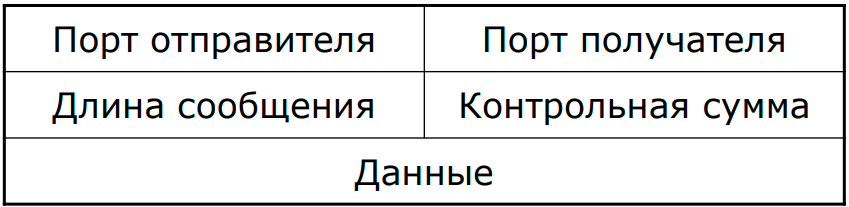
\includegraphics[width=15cm]{images/03/01}
\end{figure}

Длина сообщения~--- длина UDP дейтаграммы.

Контрольная сумма считается по всему пакету (а в IP только по заголовку).

Если контрольная сумма равна 0, то она не вычислялась (например, если мы верим, что у нас сверхнадёжный канал).

Контрольная сумма вычисляется с учётом псевдозаголовка.

\begin{figure}[H]
  \centering
  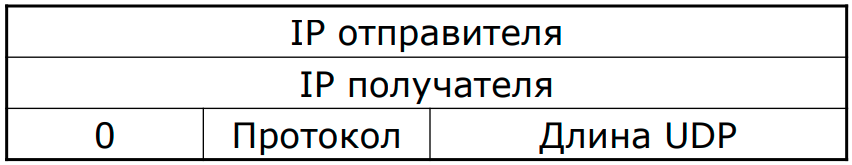
\includegraphics[width=15cm]{images/03/02}
\end{figure}

Благодаря этому, если у нас была произведена атака и были подменены IP-адреса, а контрольную сумму злоумышленник не пересчитал, то она не сойдётся (скорее всего).

Поэтому злоумышленнику нужно сохранить к себе весь пакет и пересчитать контрольную сумму (ага, очень большая проблема для него).

Приложения, использующие UDP:
\begin{itemize}
    \item TFTP (69)
    \item DNS (53)
    \item SNMP (161, 162)~--- протокол управляющих сообщений
    \item BOOTP, DHCP (67, 68)~--- получение параметров IP
    \item RIP (520)~--- маршрутизация
\end{itemize}

\Subsection{Протокол TCP}

Transmission Control Protocol

По сравнению с UDP имеет:
\begin{itemize}
    \item Более низкую скорость
    \item Большую надёжность
\end{itemize}

Зарезервирован номер 6 в IP-пакете.

Адресация с помощью TCP-портов.

Передача~--- потоковая. Данные для передачи хранятся в буфере. Это единственный протокол, который имеет дело не с пакетами, а с двумя очередями: буфером приёма и передачи. В отличие от UDP, оперируем сегментами, а не пакетами. Можем захотеть передать 100 байт, но они добавятся в общую очередь и за раз передастся 1000 байт.

Данные добавляются в конец буфера, а передаются из начала. 

Каждый передаваемый байт пронумерован. Сегменту присваивается номер его первого байта (номер очереди).

При посылке в сеть сегмента, он копируется в буфер повторной передачи, заводится таймаут. Если в течение таймаута не получили подтверждение, посылаем снова. И так делается (по дефолту) до 5 раз.

Каждый переданный байт должен быть подтверждён. При получения подтверждения от сегмента, подтверждёнными считаются все байты сегмента. Подтверждение содержит номер следующего ожидаемого байта.

\begin{figure}[H]
  \centering
  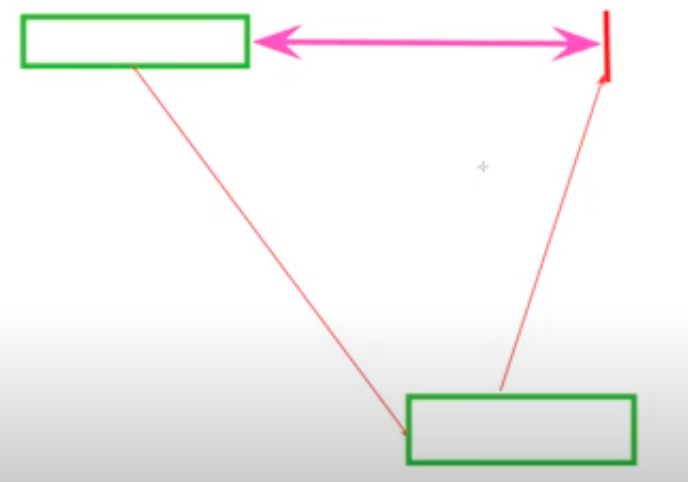
\includegraphics[width=15cm]{images/03/03}
\end{figure}

В момент времени $T_1$ Алиса послала сообщение Бобу.

В момент времени $T_2$ Боб это сообщение получил и отправил подтверждение Алисе.

В момент времени $T_3$ Алиса получила подтверждение от Боба и может отправлять второй пакет. Таким образом, мы получили простой передачи $T_3-T_1$.

В TCP отрицательные квитанции не посылаются. Например, если у нас не сошлась контрольная сумма, нам не пошлют сообщение об ошибке. Принимающая сторона просто не будет посылать подтверждение получения и мы попробуем отправить пакет снова.

\Subsubsection{Формат TCP пакета}

\begin{figure}[H]
  \centering
  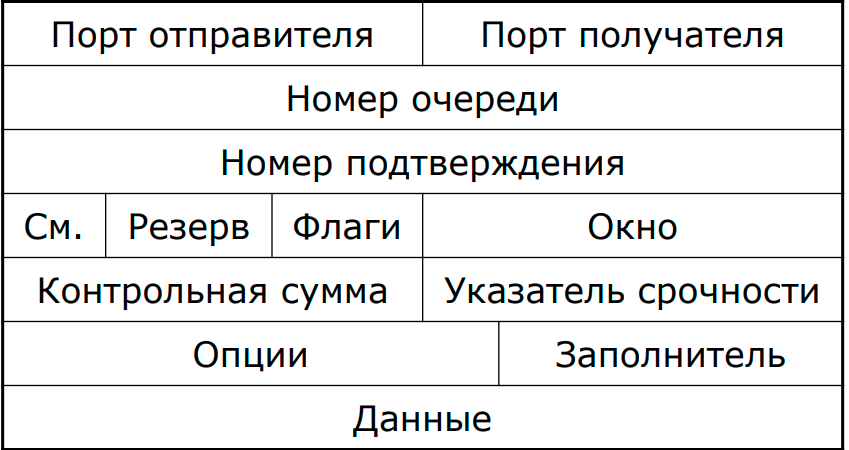
\includegraphics[width=15cm]{images/03/04}
\end{figure}

\begin{itemize}
    \item Номер очереди~--- номер посланного сегмента при обмене или синхронизация номеров сегментов при установлении соединения
    \item Номер подтверждения~--- подтверждение принятого сегмента или синхронизация номеров сегментов при установлении соединения
    \item Смещение данных~--- длина заголовка TCP (и так же, как и в IP, с помощью него понимаем, есть у нас опции или нет)
    \item Окно~--- величина скользящего окна (о нём позже)
    \item Контрольная сумма~--- по всему высылаемому сегменту
    \item Указатель срочности~--- объём срочных данных

\end{itemize}

{\bf Флаги}

\begin{figure}[H]
  \centering
  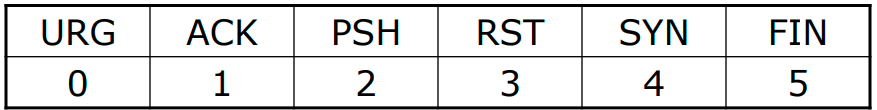
\includegraphics[width=15cm]{images/03/05}
\end{figure}

\begin{itemize}
    \item URG~--- флаг срочности. Задействовано поле <<Указатель срочности>>. Это позволяет передать определённый объём данных в сеть без буферизации. Пример, когда надо: управление удалённым терминалом, компьютерные игры.
    \item ACK~--- флаг подтверждения. Задействовано поле <<Подтверждение>> и в этом пакете у нас находится квитанция.
    \item PSH~--- флаг проталкивания. О нём позже.
    \item RST~--- флаг сброса. Перезагрузка соединения
    \item SYN~--- флаг синхронизации. Синхронизация номеров очередей для создания виртуального канала. Первый пакет с каждой стороны должен иметь установленным этот флаг
    \item FIN~--- флаг закрытия соединения. Завершение соединения
\end{itemize}

\Subsubsection{Установка соединения}

Хотим начать соединение. Нужно договориться, с какого номера клиент и сервер будут начинать отсчёт отправляемых сообщений. Казалось бы, можно начать с нуля (сначала даже так и делали), но выяснилось, что так хакерам проще вклиниться в уже установленное TCP соединение.

Поэтому решили номер первого сегмента генерировать случайно. 

Таким образом, вся установка соединения~--- двусторонний обмен номерами сегментов между отправляющей и принимающей сторонами.

\begin{enumerate}
    \item A посылает B пакет с флагом SYN, в котором указан номер первого сегмента минус единица ($N_{seqA}$)
    \item B посылает в ответ пакет с флагом ACK и $N_{ackB}=N_{seqA}+1$
    \item B посылает A пакет с флагом SYN и $N_{seqB}$
    \item A посылает B подтверждение о синхронизации с флагом ACK и $N_{ackA}=N_{seqB}+1$
\end{enumerate}

С этого момента каждый знает номер очереди собеседника и можно проводить штатный обмен.

{\bf НО!} в пакетах, отсылаемых в сообщениях 2 и 3 нет общих полей. Поэтому решили это передавать одним пакетом.

Это называется трёхпутевой схемой организации соединения.

\Subsubsection{Разрыв соединения}

\begin{enumerate}
    \item A посылает B пакет с флагом FIN
    \item B посылает A пакет с флагом ACK 
    \item B посылает A пакет с флагом FIN
    \item A посылает B пакет с флагом ACK
\end{enumerate}

\Subsubsection{Конечный автомат протокола TCP}

Как работает TCP:

\begin{itemize}
    \item На сервере есть сокет (допустим, на порту 80).
    \item Когда приходит запрос на соединение, порождается ещё один сокет (с тем же номером порта)~--- рабочий. И именно с ним работает клиент. А прошлый сокет остался в состоянии слушания входящих соединений.
    \item У рабочего сокета может быть несколько состояний.
    \item Стоит заметить, что ничего страшного в том, что у рабочего сокета такой же номер порта нет, так как сокет определяется ещё и IP-адресом клиента.
\end{itemize}

\begin{figure}[H]
  \centering
  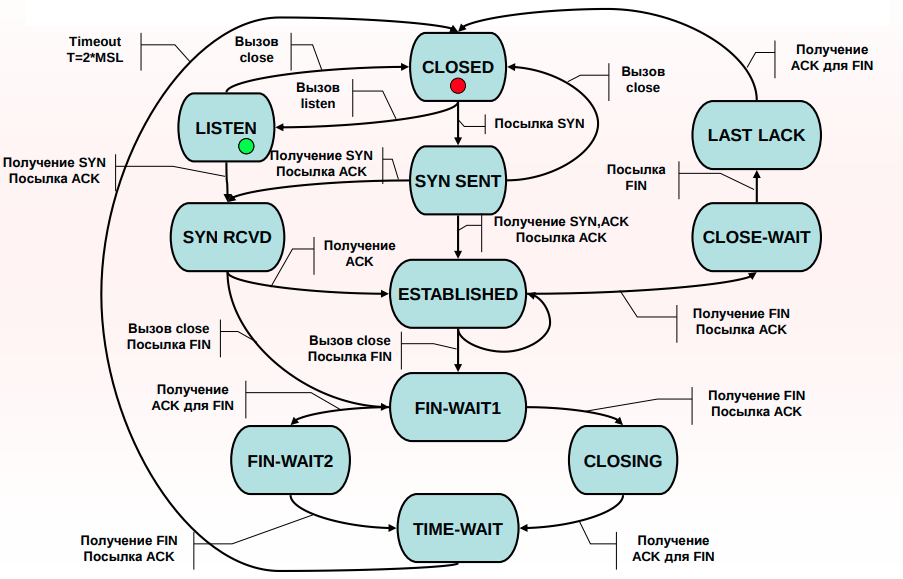
\includegraphics[width=15cm]{images/03/06}
\end{figure}

На сервере решили организовать слушающий сокет. Сделали системный вызов listen. Сокет перешёл в состояние LISTEN.

Если получили сигнал SYN, у нас породился второй сокет, красный продолжает слушать, а зелёный переходит в состояние SYN RCVD.

Получили ACK и перешли в состояние ESTABLISHED. В этом состоянии происходит вся передача данных. Все остальные состояния~--- служебные.

Пусть мы вызвали {\tt close}. Тогда перейдём в состояние FIN-WAIT1, получим ACK, перейдём в FIN-WAIT2, получим FIN, отправим ACK, перейдём в TIME-WAIT. Это долгое состояние, в котором мы разгребаем весь мусор из сети. Там ждём от полутора до трёх минут, собирая все приходящие данные, после чего переходим в CLOSED.

Есть утилита {\tt netstat}, которая позволяет посмотреть на сокеты и их состояния. Там скорее всего вы увидите толко LISTEN, ESTABLISHED и TIME-WAIT. Все остальные состояния очень быстрые.

Это было для сервера. А клиент посылает SYN, переодит в SYN SENT, ну а дальше всё так же.

\Subsubsection{Срочные данные}

URG~--- немедленная доставка данных приложению на приёмной стороне.

URG~--- флаг наличия срочных данных.

Offset~--- указатель на первые несрочные данные.

Проталкивание данных~--- немедленная отсылка сегмента в сеть. 

\Subsubsection{Управление скоростью передачи}

Идея: давайте передавать не один, а несколько сегментов и будем ждать от всех них подтверждения.

В сеть могут передаваться сегменты, которые попали в {\bf скользящее окно}.

Обычно скользящее окно кратно размеру сегмента.

Сдвиг окна происходит, когда получаем подтверждение на первый посланный сегмент.

Хотим послать в сеть 4 сегмента. И скользящее окно их покрывает. Посылаем сразу 4 сегмента и ждём подтверждений. 

Пришло подтверждение на первый сегмент~--- сдвигаем окно на величину подтверждённых данных.

Если пришло подтверждение на более поздний сегмент, это запоминается, но окно не сдвигается, пока не пришло подтверждение на самый левый из неподтверждённых сегментов.

Идеальная ситуация~--- когда подтверждение на первый сегмент приходит ровно тогда, когда мы отправили последний. Если мы так подобрали размер скользящего окна, то мы достигли максимальной возможной скорости передачи по TCP.

По ходу передачи размер окна меняется. Это всё настраивается в опциях.

{\bf Кулстори.} Раньше предлагали скачать приложения, которые ускорят ваш интернет. В 99\% случаев это были троянские кони, а 1\%~--- утилита, которая оценивала скорость связи и прописывала в реестр оптимальный размер скользящего окна.

\Subsubsection{Протоколы, использующие TCP}

\begin{itemize}
    \item telnet (23)~--- удалённый терминал
    \item SMTP (25)~--- почта
    \item FTP (20, 21)~--- передача файлов
    \item DNS (53)
    \item HTTP (80)
    \item POP3 (110)
    \item IMAP4 (143)
    \item SSH (22)
    \item ...
\end{itemize}

\Subsection{Протокол SCTP}

Stream Control Transmission Protocol

Хочется:
\begin{itemize}
    \item Объединить достоинства UDP и TCP
    \item Исправить недостатки UDP и TCP
\end{itemize}

Он позволяет внутри одного соединения организовывать несколько потоков.

Пакет состоит из заголовка и нескольких субпакетов (чанков).

\begin{figure}[H]
  \centering
  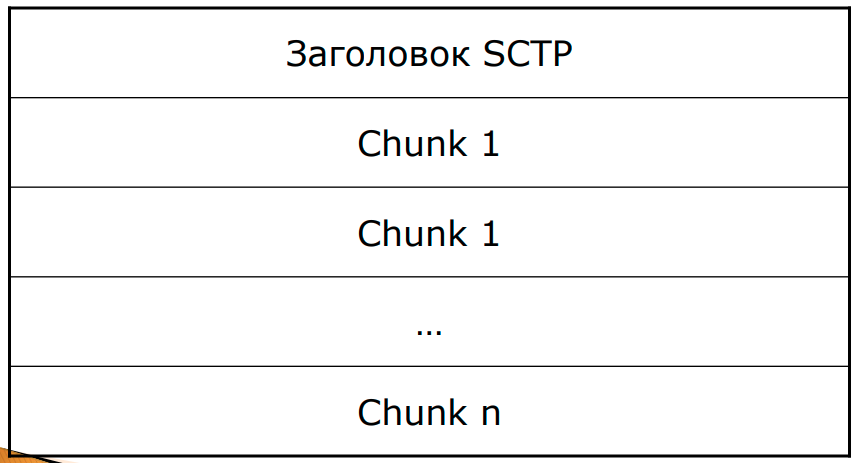
\includegraphics[width=15cm]{images/03/07}
\end{figure}

Каждый субпакет имеет свой заголовок и данные

Зачем может понадобится несколько потоков? Когда мы передаём данные разного размера, разного назначения, разной скорости.

Например, по одному передаём громадные файлы, по второму~--- сообщения, по третьему~--- управляющие команды.

По сути мы заменяем несколько TCP сокетов на один SCTP.

Формат заголовка:

\begin{figure}[H]
  \centering
  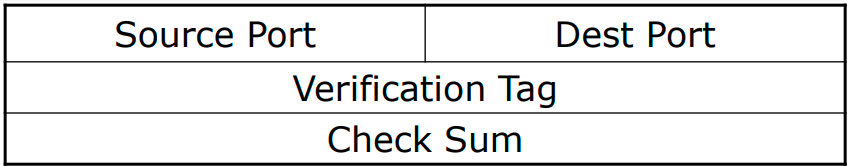
\includegraphics[width=15cm]{images/03/08}
\end{figure}

Verification Tag~--- метка для проверки отправителя пакета. Замена аутентификации.

Формат субпакета:

\begin{figure}[H]
  \centering
  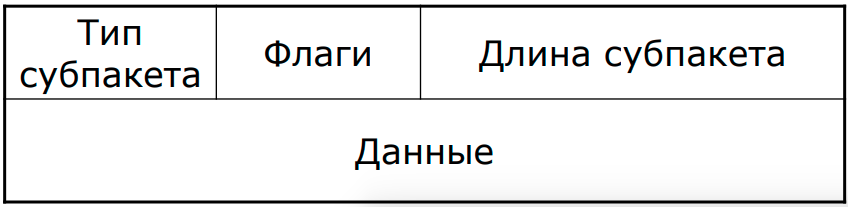
\includegraphics[width=15cm]{images/03/09}
\end{figure}

Тип субпакета~--- число от 0 до 255
\begin{itemize}
    \item 0~--- полезные данные
    \item >0~--- служебная информация
\end{itemize}

Флаги~--- служебные разряды. Определяются типом субпакета.

Особенности:
\begin{itemize}
    \item Многопоточность
    \item Мультидомность~--- SCTP может использовать сразу несколько каналов. Например. если один вышел из строя, можем использовать другой.
    \item Проверка подлинности
    \item Подтверждение приёма
    \item Средства устранения перегрузок
    \item Передача пакетами (а не как в TCP)
\end{itemize}

\Section{Маршрутизация}{Лекции 4-5}{Игорь Смирнов}

Маршрутизация~--- функция сетевого уровня.

Это процесс доставки пакетов через сеть от одного узла до другого, когда эти узлы не соединены между собой непосредственно.

Муаршрутизация бывает индивидуальной и групповой. Мы будем говорить только про индивидуальную.

Ключевая точка обмена трафиком в СПб~--- на Марсовом поле, в здании компании Ленэнерго.

\Subsection{Маршрутизаторы}

Это устройство сетевого уровня, реализующее функции маршрутизации (обеспечивающее доставку пакетов от одного узла сети к другим).

Другие названия маршрутизаторов:
\begin{itemize}
    \item Шлюз
    \item Router
    \item Gateway
\end{itemize}

Маршрутизатор отличается от конечного узла тем, что он пересылает входящие пакеты, у которых адрес назначения не совпадает с локальным адресом узла. Это называется {\bf IP-forwarding}.

Виды маршрутизаторов:
\begin{itemize}
    \item Аппаратные (маршрутизатор, router)
    \begin{itemize}
        \item Поддержка различных канальных сред
        \item Несколько сетевых интерфейсов
        \item Высокая производительность
        \item Высокая надёжность
        \item Хорошая защищённость
        \item Дополнительные функции: фильтрация, трансляция адресов, сбор статистики
        \item Обычно высокая стоимость
    \end{itemize}
    \item Программно-аппаратные (шлюз, gateway)
    \begin{itemize}
        \item Реализуются функциями ОС общего назначения
        \item Характеризуются невысокой производительностью, невысокой стоимостью
        \item Могут совмещать функции с обычными функциями ОС
    \end{itemize}
\end{itemize}

Процесс маршрутизации:

\begin{figure}[H]
  \centering
  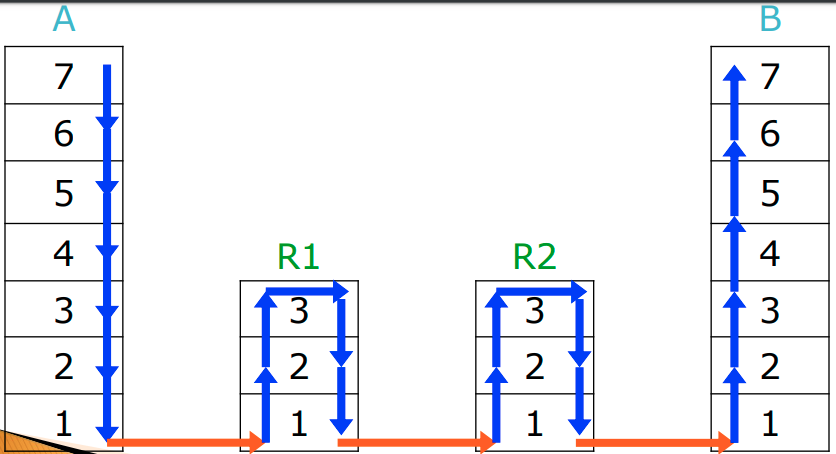
\includegraphics[width=15cm]{images/04/01}
\end{figure}

Маршрутизатор поднимает пакет до сетевого уровня. Если пакет предназначался не ему, посылает следующему маршрутизатору.

\Subsection{Виды маршрутизации}

\begin{itemize}
    \item По адаптивности:
    \begin{itemize}
        \item Статическая
        \item Динамическая
        \item <<От источника>>
    \end{itemize}
    \item По месту маршрутных вычислений:
    \begin{itemize}
        \item Централизованные
        \item Децентрализованные
    \end{itemize}
    \item По требуемой информации:
    \begin{itemize}
        \item Локальные
        \item Глобальные
        \item Смешанные
    \end{itemize}
\end{itemize}

(это всё уже было, поэтому пояснять не буду)

\Subsection{Таблицы маршрутизации}

О том, как они создаются, поговорим отдельно.

Таблицы маршрутизации состоят из:
\begin{itemize}
    \item Атрибутов маршрутных записей
    \begin{itemize}
        \item Сеть/узел назначения
        \item Сетевой интерфейс (через который нужно посылать на этот узел/сеть)
        \item Маршрутизатор (адрес)
        \item Метрика маршрута (стоимость маршрута)
        \item Флаги (каким образом маршрут был получен)
    \end{itemize}
    \item Псевдомаршрутов
    \begin{itemize}
        \item Дополнительные записи в таблице маршрутизации
        \item Используются для унификации процедуры поиска маршрута
        \item Бывают двух типов: на IP-адреса собственных сетевых интерфейсов и на подключённые IP-сети. Ни в одном, ни в другом случае реальная маршрутизация не нужна, поскольку доставка делается в рамках канальной сети. Но для унификации они добавлены в таблицу маршрутизации.
    \end{itemize}
\end{itemize}

Маршрут <<по умолчанию>>~--- маршрут, который выбирается, если ни одна из наших записей не подошла для входящей дейтаграммы.

Обозначается {\tt 0.0.0.0/0.0.0.0} (по сути это обозначение всей сети Internet). 

Управлять таблицей маршрутизации можно с помощью утилиты route.

Пример таблицы маршрутизации:

\begin{figure}[H]
  \centering
  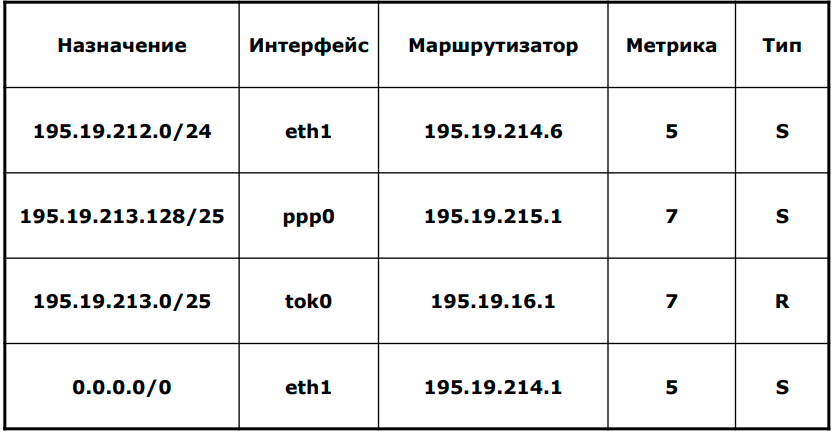
\includegraphics[width=15cm]{images/04/02}
\end{figure}

В классической маршрутизации адрес источника вообще не используется. Но, например, провайдерам это бывает нужно. Например, у нас есть дорогой клиент, который требует определённого уровня качества и есть дешёвый клиент, которому мы не гарантируем скорость доставки. Тогда дорогого клиента можно отправлять по <<чистому>> пути.

По умолчанию, TCP/IP поддерживает только одну таблицу маршрутизации. Но в некоторых системах поддерживается несколько таблиц маршрутизации.

В этих системах в зависимости от адреса источника выбирается подчинённая таблица маршрутизации, а в ней уже маршрутизация по адресу приёма.

Так можно решать задачу о балансировке трафика, например.

\Subsection{Статическая маршрутизация}

Все маршруты создаются вручную администратором, хранятся в таблицах до выключения.

\begin{figure}[H]
  \centering
  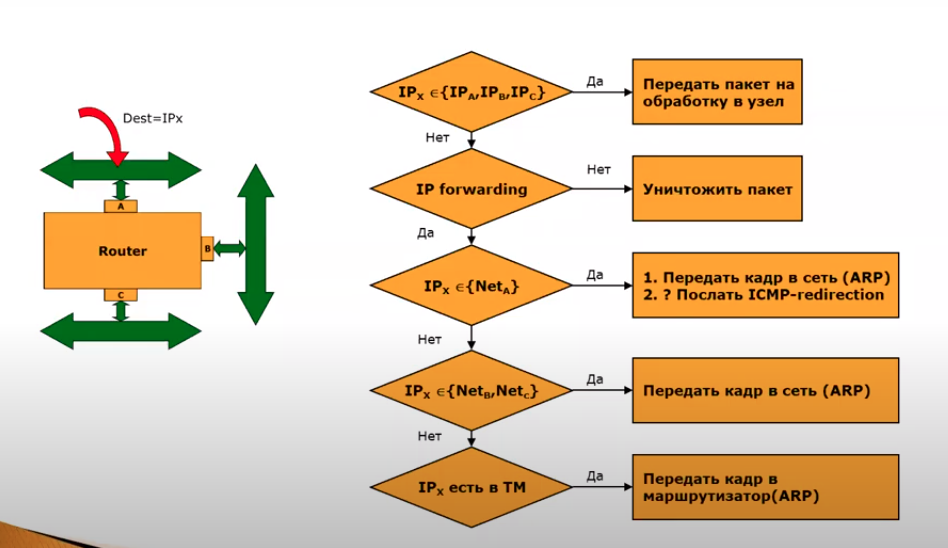
\includegraphics[width=15cm]{images/04/03}
\end{figure}

Псевдомаршруты помогают убрать 3 и 4 ромбики. Мы считаем, что это такие же адреса и маршрутизируем их по тому же правилу, что и 5. (оптимизации, которые мы заслужили)

\Subsection{Динамическая маршрутизация}

Статическая маршрутизация никак не зависит от ситуации в сети. Каналы связи могут обрываться, добавляться новые, маршрутизаторы могут выходить из строя...

{\bf Куллстори.} Основная причина сбоев интернета в России~--- экскаватор порвал волокно.

Что меняется в сети:
\begin{itemize}
    \item Топология
    \begin{itemize}
        \item Появление новых узлов
        \item Появление новых каналов
        \item ...
    \end{itemize}
    \item Каналы связи
    \begin{itemize}
        \item Выход из строя канала
        \item Ввод в строй канала
    \end{itemize}
    \item Узлы сети
    \begin{itemize}
        \item Выход из строя маршрутизатора
        \item Ввод в строй маршрутизатора
    \end{itemize}
    \item Нагрузка
\end{itemize}

\Subsection{Алгоритмы динамической маршрутизации}

Задача оптимальной маршрутизации~--- найти оптимальный путь для пакета в данный момент времени.

Поиск оптимального маршрута~--- поиск кратчайшего пути на графе.

Узлы графа~--- маршрутизаторы, дуги~--- каналы, веса~--- метрика.

Под оптимальностью можно понимать разные вещи:
\begin{itemize}
    \item Минимальное время доставки
    \item Минимальная стоимость доставки
    \item Минимальная задержка
    \item ...
\end{itemize}

Из алгоритмов используют Форда-Беллмана и Дейкстру и их модификации.

Расписывать ФБ и Дейкстру не буду.

ФБ работает за $\O(V^3)$ (это, конечно, правда, но аааааааа, $\O(VE)$ же... Или сеть~--- это почти полный граф?), но у нас ФБ с break, поэтому он работает более-менее норм. А ещё он легко параллелится.

Это локальный алгоритм (то есть нам не нужно знать топологию всей сети (а почему это так~--- увидим позже)).

{\bf Куллстори.} Дейкстра получил премию имени Дейкстры. Он создал эту премию, умер, премию переименовали в его честь и дали ему посмертно.

Время работы Дейкстры $\O(V^2)$.

Тут, в отличие от ФБ, нам нужно знать топологию всей сети. А ещё Дейкстра не очень хорошо параллелится.

Дейкстра требует $\O(V^2)$ памяти <<на хранение всей матрицы расстояний>> и это проблема при больших $V$ (тут был пример про $V\approx 10\,000$, но блин, ну правда же, что граф такой сети обычно прямо совсем не полный?..) 

\Subsection{Системы маршрутизации}

AS~--- автономная система.

Имеет уникальный номер.

AS:
\begin{itemize}
    \item Часть сети, управляющаяся из одного центра управления
    \item Реализующая одну политику маршрутизации
    \item Внутри AS обеспечиваются одинаковые протоколы маршрутизации
\end{itemize}

То есть это такой локальный центр управления маршрутизацией в интернете.

\begin{figure}[H]
  \centering
  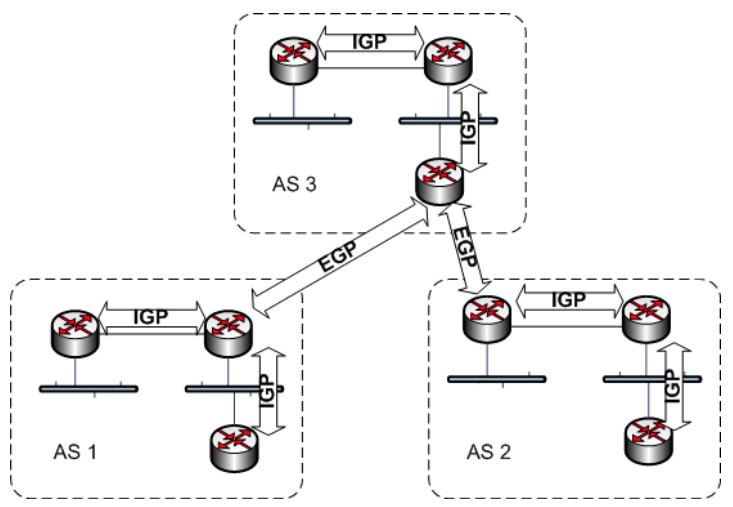
\includegraphics[width=15cm]{images/04/04}
\end{figure}

Протоколы маршрутизации внутри AS~--- внутренние (IGP~--- Interior Gateway Protocol), между AS~--- внешние (EGP~--- Exterior Gateway Protocol).

Некоторые маршрутизаторы являются пограничными и обеспечивают связь между разными AS.

\Subsubsection{Протоколы маршрутизации}

Характеристики:
\begin{itemize}
    \item Название 
    \item Стандартизирующие документы
    \item Алгоритм поиска маршрута
    \item Метрика протокола
    \item Сходимость~--- способность протокола оперативно реагировать на изменения в сети и приводить маршрутизаторы к соответствующее состояние\\
    Время сходимости – время за которое маршрутные таблицы переходят в состояние, адекватное изменившейся ситуации сети
    \item Избежание петель маршрутизации
    \item Загрузка сети
    \item Ресурсоёмкость
    \item Поддержка нескольких маршрутов на сеть (однопутевые или многопутевые)
    \item Аутентификации
    \item Ограничения применения
    \item Конфигурирование
    \item Поддержка в маршрутизаторах
\end{itemize}

\Subsubsection{Метрики маршрутов}

Метрика может зависеть от:
\begin{itemize}
    \item Числа промежуточных маршрутизаторов
    \item Пропускной способности канала связи
    \item Задержек в канале связи
    \item Надежности канала связи
    \item Загрузки канала связи
\end{itemize}

В общем случае, метрика моет быть комбинацией этих параметров.

\Subsection{Внутренние протоколы маршрутизации}

\begin{itemize}
    \item RIP
    \item OSPF
    \item IGRP
    \item EIGRP
    \item IS-IS
    \item ...
\end{itemize}

\Subsubsection{Протокол маршрутизации RIP}

Routing Information Protocol

Используется в TCP/IP и Novell

Использует ФБ.

Тип протокола~--- однопутевой. То есть может хранить только один путь на целевую сеть.

Самая слабая его сторона~--- метрика. В нём это целое число от 0 до 15, которое означает число промежуточных маршрутизаторов до сети назначения. Для соседей~--- 0, 16~--- сеть недоступна.

Эта метрика не зависит от задержек, пропускной способности, надёжности, загрузки.

Граф для ФБ~--- с единичными весами рёбер.

Алгоритм функционирования RIP:
\begin{enumerate}
    \item Рассылка соседям маршрутной информации (по сути рассылаем соседям свою таблицу маршрутизации со своими текущими расстояниями). Это происходит раз в 30 секунд
    \item Корректировка собственной ТМ после получения обновления от соседей (по сути тоже получаем их таблицы маршрутизации и текущими расстояниями)
\end{enumerate}

{\bf Корректировка таблицы:}

\begin{figure}[H]
  \centering
  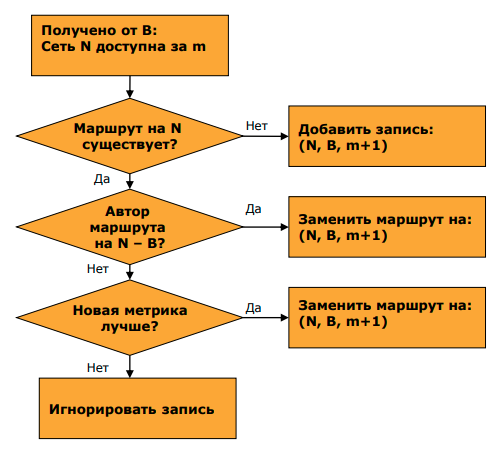
\includegraphics[width=15cm]{images/04/05}
\end{figure}

При корректировке, если к нам прислали новый маршрут, мы должны не просто сделать {\tt min=}.

Допустим, узел B говорит, что сеть N доступна за m шагов. Если наш путь на N проходил через B, то мы в любом случае должны обновить расстояние, даже если оно стало хуже, потому что B лучше знать, какой путь до N (мало ли там что-то испортилось).

При этом мы на каждый маршрут в таблице заводим таймер. Если больше трёх минут сосед нам ничего не посылает, то мы по прежнему используем его для маршрутизации, но уже не рассылаем соседям.

А если сосед нам ничего не посылает больше 5 минут, то мы удаляем этото маршрут из нашей таблицы маршрутизации.

{\bf Петли маршрутизации}

Пусть сеть A подключена к сети B, а та непосредственно подключена к сети N.

И вдруг внезапно кабель до сети N порвался и она перестала быть доступна. Тогда обновляться таблицы маршрутизации будут как показано на картинке:

\begin{figure}[H]
  \centering
  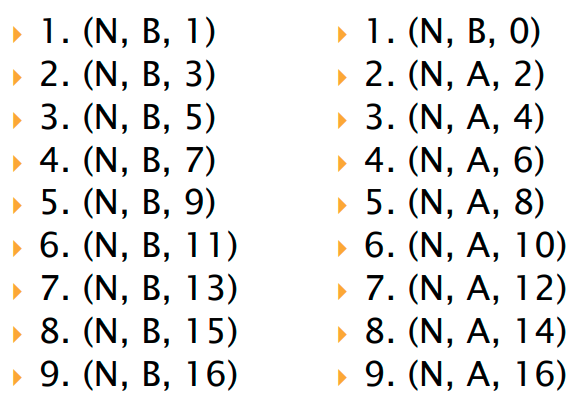
\includegraphics[width=15cm]{images/04/06}
\end{figure}

И только на 9 шаге мы поймём, что сеть N недоступна. То есть мы только через 5 минут узнаем об этом. А всё это время пакеты будут гоняться между A и B и умирать по TTL. Это, к тому же, загружает сеть. Печально.

Чтобы бороться со всем этим, придумали несколько технологий преодоления петель маршрутизации. {\it А что самое главное в технологии преодоления? Хорошее название.}
\begin{itemize}
    \item Split Horizon~--- расщепление горизонта.\\
    Обновления не посылаются на тот интерфейс, из которого этот маршрут получен. 
    \item Poison Reverse~--- обратный яд\\
    Обновления маршрута посылаются на интерфейс, из которого этот маршрут получен, но с метрикой 16
    \item Triggered Updates~--- мгновенные обновления\\
    Если в сети происходит какое-то изменение, то забываем про 30-секундные интервалы и начинаем сразу передавать информацию.\\
    Ускоряется сходимость протокола, но при этом лавинообразно увеличивается трафик.
    \item Hold Down\\
    Кратковременное прекращение приема обновлений маршрута после получения его обновления от автора с метрикой 16\\
    В течение 120 с маршрутизатор не принимает обновления этого маршрута, пережидая переходные процессы в сети\\
    {\it <<Когда мы кидаем камни в воду, некоторое время круги расходятся. Идея Hold Down: давайте переждём эти переходные процессы в сети>>}
\end{itemize}

На практике используют сразу несколько из этих технологий. 

{\bf Никакие технологии не спасают от петли маршрутизации, включающей более 2 узлов.}

{\bf Транспортировка данных в RIP.}

Соседние маршрутизаторы~--- широковещательно.

Рассылка обновлений: {\tt 255.255.255.255} (все узлы данной локальной сети).

RIP инкапсулируется в UDP (порт 520).

В один пакет входит до 25 маршрутных записей. Максимальная длина пакета~--- 512 байт.

Формат пакета:

\begin{figure}[H]
  \centering
  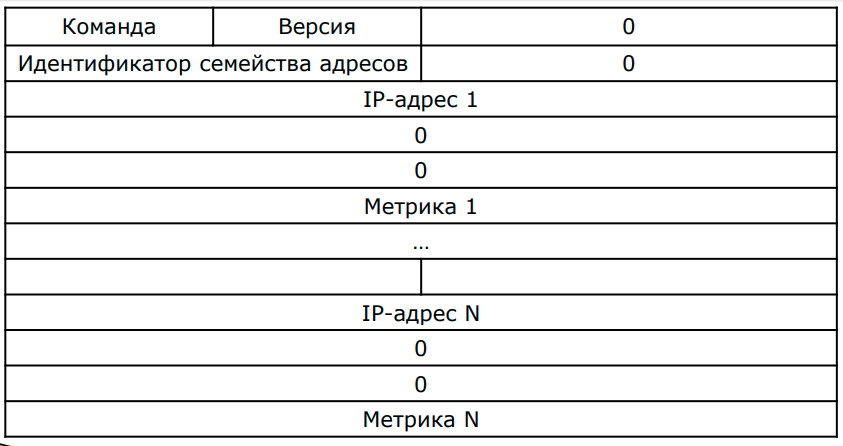
\includegraphics[width=15cm]{images/04/07}
\end{figure}

\begin{itemize}
    \item Команда~--- код операции (1~--- запрос, 2~--- ответ)\\
    Запрос нужен, если у нас появилась новая станция. Она не ждёт 30 секунд, а сразу посылает запрос, чтобы ей скинули таблицы маршрутизации.
    \item Идентификатор семейства адресов~--- тип сетевой среды (для TCP/IP~--- 2)
    \item IP-адрес~--- адрес сети класса A, B или C. То есть RIP не поддерживает подсети.
\end{itemize}

Итого: RIP~--- простой протокол, у него низкие требования к вычислительным ресурсам и объёмам памяти, легко настраивается (работает из коробки, но можно указать алгоритмы обхода петель и интерфейсы).

Но при этом плохая метрика, высокая нагрузка сеи, ограниченный диаметр сети (15), медленная сходимость, не поддерживает маски подсети, нет подтверждения подлинности и шифрования.

{\bf Куллстори.} В 95 году на кафедре Политеха только появились компьютерные сети. И стала происходить странная ситуация: каждый четверг в 12:00 интернет отключался и переставал работать. А в 13:40 всё включалось и продолжало работать. Проблема была в следующем: на одном из кафедральных маршрутизаторов, подключённых к общей сети, был некорректно настроен сервис маршрутизации. Когда этот компьютер включали, он сообщал всем, что у него есть маршрут на сеть {\tt 0.0.0.0} с метрикой 0. Все перестраивали путь на него. А почему это происходило раз в неделю? Потому что интернет тогда был по расписанию, преподаватель в 12:00 приходил на работу, включал сервер, полтора часа вёл занятия и выключал его.

\Subsubsection{протокол маршрутизации RIP-II}

Появилась аутентификация, маска сети, групповая адресация вместо широковещательной, добавились метки маршрута и ссылка на следующий маршрутизатор.

Групповая адресация (по {\tt 224.0.0.9}) лучше широковещательной тем, что в широковещательной этот пакет получат все узлы, а тут только маршрутизаторы, использующие RIP.

Формат пакета:

\begin{figure}[H]
  \centering
  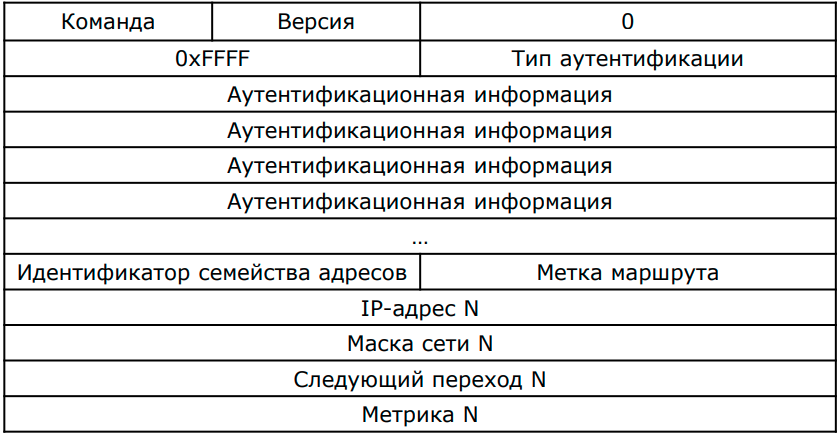
\includegraphics[width=15cm]{images/04/08}
\end{figure}

<<Следующий переход>> нужен для исключения лишних шагов в маршрутизации и для возможности использовать информацию из других источников (не из RIP-а).

Метка маршрута нужна для упрощения взаимодействия с EGP.

Совместим с RIP-1.

\Subsubsection{Протокол маршрутизации OSPF}

OSPF = Open Shortest Path First

Использует алгоритм Дейкстры.

Сейчас он очень широко используется.

Метрика~--- число от 0 до 65535~--- количество секунд, требуемое для передачи 100 Мбит через физическую среду данной сети
\begin{itemize}
    \item 10Base-T Ethernet – 10
    \item 56 кбит/с – 1785
    \item Метрика канала со скоростью передачи данных 100 Мбит/с и выше – 1
\end{itemize}

Для каждого канала связи метрика может задаваться администратором (если вдруг захотим трактовать метрику по-другому. Например, сейчас большинство сетей быстрее 100 Мбит/с).

Так как используется Дейкстра, мы должны всем узлам сообщить топологию. Для этого рассылаем пакеты LSA~--- Link State Advertisment. Там есть информация о каналах и их состояниях (метриках).

По сути кадый узел графа рассказывает о своих дугах.

Рассылка осуществляется только если что-то меняется. 

Рассылаются лавинным образом (то есть все шлют одновременно) и все получают информаци о всех.

Все маршрутизаторы строят LSD~--- Link State Database. ЧТобы протокол работал корректно, нужно чтобы все LSD были одинаковыми.

На основе LSD строим LST~--- Link State Tree (просто дерево Дейкстры из этой вершины).


Причины рассылки LSA:
\begin{itemize}
    \item Изменилось состояние интерфейса
    \item Произошли изменения в маршрутизаторе сети
    \item Произошло изменение состояния одного из соседних маршрутизаторов
    \item Изменилось состояние одного из внутренних маршрутов
    \item Изменение состояния межзонного маршрута
    \item Появление нового маршрутизатора, подключенного к сети
    \item Возникли изменения одного из внешних маршрутов
    \item Маршрутизатор перестал быть пограничным для данной AS (например, перезагрузился)
    \item Возраст маршрута достиг предельного значения (30 минут)
    \item ...
\end{itemize}

{\bf Таблица маршрутизации OSPF}
\begin{itemize}
    \item IP-адрес места назначения и маска
    \item Тип места назначения (сеть, граничный маршрутизатор и т.д.)
    \item Тип сервиса (TOS)~--- OSPF позволяет строить разные типы маршрутов для разных типов сервиса. 
    \item Домен маршрутизации
    \item Тип пути (внутренний; межобластной; внешний, ведущий к AS)
    \item Метрика
    \item Следующий маршрутизатор
    \item Объявляющий маршрутизатор (используется для межобластных обменов и для связей автономных систем друг с другом)
\end{itemize}

Не хочется грузить сеть лавинным трафиком. Давайте найдём в сети какой-нибудь маршрутизатор, все отправим ему, а уже он перешлёт всем. Это делают назначенные маршрутизаторы (DR~--- Designated Router).

Если он есть, то шлют LSA ему.

На всякий случай есть запасной~--- BDR (Backup Designated Router).

OSPF инкапсулируется в IP (с кодом 89).

Для передачи маршрутных обновлений используются адреса:
\begin{itemize}
    \item Для адресации всех OSPF-маршрутизаторов: {\tt 224.0.0.5}
    \item Для адресации всех назначенных OSPF-маршрутизаторов: {\tt 224.0.0.6}
\end{itemize}

В OSPF есть политика доменов маршрутизации. Если у нас есть большая сеть, то давайте разделим её на 4 подсегмента (например, мы можем захотеть это сделать, если у нас граф сети очень большой).

Внутри доменов своя маршрутизация, есть междоменная маршрутизация. 

Достоинства OSPF:
\begin{itemize}
    \item Гибкая метрика
    \item Быстрая сходимость (почти мгновенная)
    \item Низкая загрузка каналов служебным трафиком
    \item Отсутствие петель маршрутизации
    \item Поддержка доменов маршрутизации (позволяет уменьшить требования к ресурсам сети)
    \item Поддержка различных маршрутов для разных типов обслуживания (он такой единственный из тех, что мы рассмотрим. Если нужна сеть с POS, то, это, пожалуй, единственный варинат)
\end{itemize}
Недостатки OSPF:
\begin{itemize}
    \item Высокие требования к ресурсам:
    \begin{itemize}
        \item Быстродействие
        \item Объемы памяти для хранения LSD, LST
    \end{itemize}
    \item Высокая сложность конфигурирования (надо конфигурировать идентификатор домена маршрутизации, все параметры каналов связи для каждого маршрутизатора)
\end{itemize}

\Subsubsection{Протокол маршрутизации EIGRP}

Это расширение IGRP. Но IGRP не рассматриваем, потому что он устаревший.

Enhanced Interior Gateway Routing Protocol.

Разработан компанией Cisco и не регламентируется RFC (это редкость).

IGRP~--- это был продвинутый RIP, но он проигрывал OSPF.

Это гибридный протокол. Он дистанционно-векторный с элементами протокола состояния канала.

Основные особенности:
\begin{itemize}
    \item Механизм обнаружения соседей
    \item Посылка обновлений таблиц
    \item Вычисление вероятных заместителей (механизм запасных маршрутов)
    \item Алгоритм активного поиска DUAL (на случай плохого состояния в сети)
\end{itemize}

Метрика~--- самая сильная часть этого протокола.

Определяется параметрами:
\begin{itemize}
    \item Задержка (D~---Internwork delay)~--- значение в диапазоне 10 мкс~-- 167 с
    \item Ширина полосы (B~---bandwidth)~--- значение в диапазоне 1200 б/с~-- 10Гб/с (для текущих сетей {\it почти} подходит. Сейчас у самых быстрых промышленных сетей 100Гб/с)
    \item Надежность (R~---reliability)~--- определяется вероятностью успешной посылки в данном канале связи (0-1). Можно вычислять по статистике.
    \item Нагрузка (L~---load)~--- определяется долей занятости канала (0-1)
\end{itemize}

$M=(K_1\cdot B + \frac{K_2\cdot B}{256-L} + K_3\cdot D)\cdot\frac{K_5}{R+K_4}$ при $K_5\neq 0$

$M=K_1\cdot B + \frac{K_2\cdot B}{256-L} + K_3\cdot D$ при $K_5= 0$

Коэффициенты $K_{1..5}$ определяются пользователем

По умолчанию:

$K_1=K_3=1$

$K_2=K_4=K_5=0$

$M=B+D$

Задержка измеряется в 10 мкс. $D\in[1..2^{24}]$

Полоса пропускания~--- в Кбит/с. $B\in[1..2^{24}]$

Надёжность~--- доля успешно переданных и принятых пакетов. $R\in[0..255]$

Загрузка~--- занятая часть канала в процентном соотношении. $L\in[0..255]$

{\bf Механизм обнаружения соседей.}

Хотим получать информацию о соседях маршрутизатора. Для этого посылается пакет {\tt Hello} (для быстрых сетей раз в 5 секунд, для медленных раз в 60 секунд).

По получаемым сообщениям делаем выводы об имеющихся соседях (например, можем сохранять все полученные пакеты и смотреть, когда нам в последний раз с определённого IP-адреса что-то отправляли).

{\bf Таблица топологии.}

Вместо таблицы маршрутизации тут используют таблицу топологии. Она расширяет таблицу маршрутизации.

Она предназначена для выбора маршрутов на сеть назначения.

Поля:
\begin{itemize}
    \item Минимальная полоса пропускания в пути
    \item Общая задержка пути
    \item Надежность пути
    \item Загрузка пути\\
    Эти 4 параметра рассчитаны по всему каналу связи.
    \item Минимум MTU на пути
    \item Текущая дистанция~--- текущее значение метрики сети маршрута от нашего узла до сети назначения
    \item Отчетная дистанция~--- та дистанция, которую нам прислал источник, до того, как мы её увелечили на $d$ нашего канала (то есть путь без одного ребра)
    \item Источник маршрута
\end{itemize}

{\bf Выбор путей.}

Когда хотим определить отимальный маршрут, мы выбираем путь с наименьшей дистанцией.

Также выбираются запасные пути~--- вероятные заместители. Они выбираются так, чтобы отчётная дистанция была меньше текущей дистанции оптимального маршрута.

\begin{figure}[H]
  \centering
  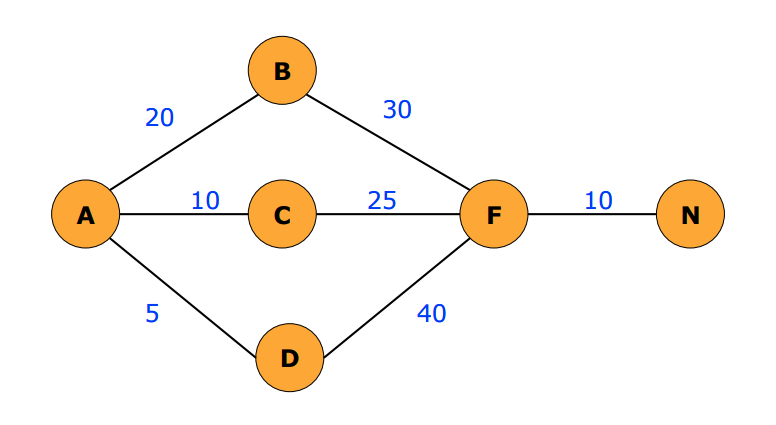
\includegraphics[width=15cm]{images/04/09}
\end{figure}

На этом примере оптимальный маршрут~--- ACF (с длиной 45).

А заместителем будет маршрут через B (потому что его отчётная дистанция~--- 40, тогда как отчётная дистанция маршрута через D~--- 50, хоть маршрут через D и короче).

Это сделано так, чтобы избежать петель маршрутизации. Посмотрим на мир глазами маршрутизатора A. Он видит только соседей и расстояния от них до N. И возможно такое, что оптимальный маршрут через D проходит обратно через A, а дальше по оптимальному маршруту для A. Тогда если оптимальный маршрут для A сломается, сломается и этот маршрут. А наше правило (отчётная длина меньше длины оптимального) гарантирует нам, что такого не случится. 

{\bf Алгоритм DUAL.}

Diffuse Update Algorithm.

Используется для активного поиска маршрута в случает удаления его из таблицы маршрутизации.

\begin{itemize}
    \item Станция, потерявшая маршрут, использует вероятного заместителя
    \item Если его нет - посылает запрос соседям
    \item Если сосед имеет вероятного заместителя~--- посылает ответ
    \item Если сосед не имеет~--- сам начинает процедуру активного поиска (для поиска использует все интерфейсы, кроме входящего)
\end{itemize}

{\bf Типы пакетов в EIGRP.}

\begin{itemize}
    \item Приветствие (Hello)
    \begin{itemize}
        \item Используется для группового оповещения соседей
        \item Не требует подтверждения
    \end{itemize}
    \item Обновление (Update)
    \begin{itemize}
        \item Если обнаружен новый сосед~--- обновление посылается индивидуально
        \item Если изменение в маршруте~--- обновление посылается по групповому адресу
    \end{itemize}
    \item Запрос (Query)~--- для DUAL
    \begin{itemize}
        \item Запросы по групповому адресу
    \end{itemize}
    \item Ответ (Reply)~--- для DUAL
    \begin{itemize}
        \item Посылаются в ответ на запрос
        \item Сообщают автору, что есть вероятный заместитель
        \item Всегда отправляются индивидуально автору запроса
    \end{itemize}
    \item Запрос информации (Request)
\end{itemize}

Метрики каналов <<по умолчанию>>:

\begin{figure}[H]
  \centering
  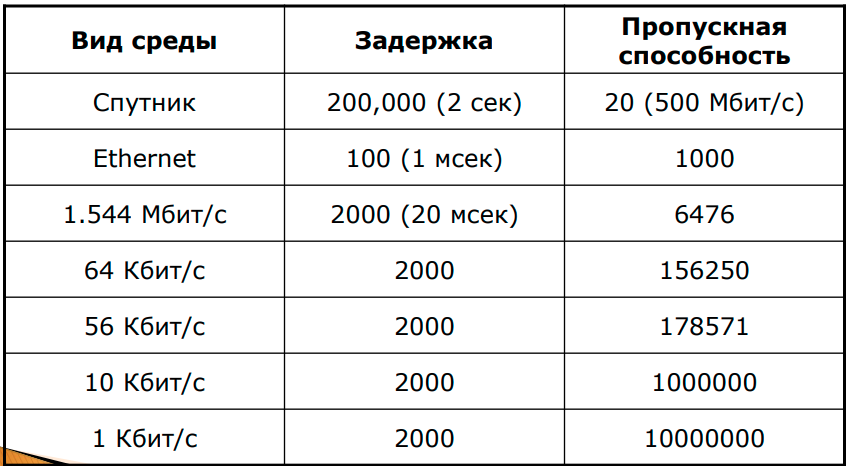
\includegraphics[width=15cm]{images/04/10}
\end{figure}

Это всё можно перенастроить.

В качестве транспорта в EIGRP используется IP (номер 9).

А ещё Cisco зачем-то получила номер 88 в IP для IGRP/EIGRP, но не использует его.

Используется широковещательный механизм рассылки маршрутных обновлений.

Достоинства EIGRP:
\begin{itemize}
    \item Очень малое использование сети в нормальном состоянии (только передача Hello)
    \item При изменениях посылаются только изменения маршрутных таблиц
    \item Низкое время сходимости
    \item Обход петель маршрутизации
    \item Поддержка маски сети
    \item Простота реализации
\end{itemize}

Недостатки EIGRP:
\begin{itemize}
    \item Несколько худшая по сравнению с OSPF сходимость
\end{itemize}

\Subsection{Протоколы внешней маршрутизации}

Нужны чтобы передавать пакеты между AS.

Всего таких протоколов два: EGP и BGP.

\Subsubsection{EGP}

External Gateway Protocol

Не имеет метрики (по сути протокол достижимости).

Единицей измерения была не одна сеть или один IP-адрес, а целая автономная система.

Сейчас уже почти не используется.

\Subsubsection{BGP}

Основан на Дейкстре.

Текущая версия~--- 4.

Используется для междоменной маршрутизации.

Оперирует тоже автономными системами.

Как транспорт использует TCP (порт 179). Это единственный протокол маршрутизации, использующий TCP.

В жизни мы его встретим максимум в одном случае~--- если будем работать у провайдеров первого уровня.

Вообще, ещё есть протокол ES-IS, но он вообще не используется.



\Section{Доменная система имён}{Лекции 5-6}{Игорь Смирнов}

У систем именования ресурсов есть несколько функций.

Основные:
\begin{itemize}
    \item Преобразование символических имен (какой-то удобной мнемоники для человека) в адреса
    \item Преобразование адресов в символические имена
\end{itemize}

Дополнительные:
\begin{itemize}
    \item Маршрутизация почты
    \item Хранение дополнительной информации об узлах
\end{itemize}

Когда интернет только появился, для именования узлов использовали таблицы соответствий.

Это был файл {\tt hosts}, в котором было соответствие имён и адресов. Первые сети так и работали.

Но такая схема долго прожить не смогла. Как только появлялся новый узел, он регистрировался и новый файл hosts рассылался всем. Это неудобно. И информация постоянно меняется.

Предложили выход~--- распределённую базу данных соответствий.

Таким образом была разработана система DNS.

Основные особенности:
\begin{itemize}
    \item Распределённая по Internet база данных имён
    \item Иерархическое именование ресурсов
    \item Распределенные по сети серверы DNS, осуществляющие запросы к распределенной базе данных DNS
\end{itemize}

Система DNS~--- это дерево. У него есть корень, который называется <<.>>. Внутрь домена верхнего уровня могут вкладываться домены следующего уровня. Количество уровней иерархии~--- неограниченно. Полное имя узла получается восстановлением по дереву снизу вверх цепочки имен доменов, разделенных точками.

Любое правильное имя в сети Internet должно заканчиваться на точку. Но почти всегда можно точку не писать.

\Subsection{Доменные имена}

Иерархия имён в DNS:

\begin{figure}[H]
  \centering
  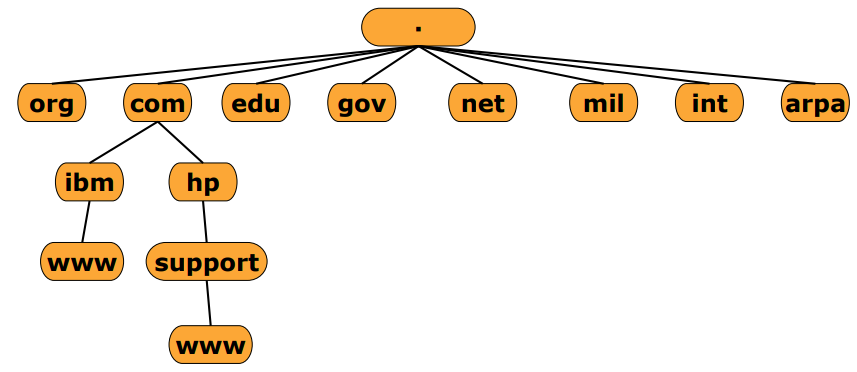
\includegraphics[width=15cm]{images/05/01}
\end{figure}

arpa~--- устаревший домен, используется для управления в Internet.

После того как интернет перестал быть американским, были добавлены национальные домены первого уровня (двухбуквенные country-коды). Например, {\tt fr, de, ca, ru, uk, ua, su (Soviet Union!)}.

{\bf Куллстори.} Есть домен {\tt tv} и он принадлежит Тувалу. Основной доход Тувалу~--- сдача домена tv под использование телевизионным компаниям.

Изначально us и su были географическими доменами. Идея была такая: в других доменах можно заводить поддомены как хотите, а в этих только с географическим принципом. Например, в us поддомены~--- названия штатов, а у них поддомены~--- названия городов. То есть если хотите обратиться в мэрию Нью-Йорка, думать не надо, просто вбиваете {\tt gov.ny.us}.

Но теперь в домене su можно регистрировать что угодно.

А ещё появились дополнительные домены первого уровня (asia, aero, biz, cat (нет, не для котеек, а для каталанского языкового и культурного сообщества), eco, info, museum, name, travel ...)

Несколько лет назад было принято решение снять ограничения с регистрации доменов первого уровня.

В том числе, это ограничение сняли из-за того, что слишком много всего было на домене {\tt com}.

Но некоторые имена всё-таки нельзя использовать в качестве доменов:
\begin{itemize}
    \item example~--- зарезервировано для примеров (например, на лекциях) 
    \item invalid~--- зарезервировано для использования в очевидно неверных именах доменов 
    \item localhost~--- зарезервировано для того чтобы избежать конфликтов с традиционным использованием localhost
    \item test — зарезервировано для использования в тестах
    \item * local, * localdomain для адресов, применяемых в пределах одной машины или локальной компьютерной сети
\end{itemize}

\Subsubsection{Правила построения доменных имён}

Используемые символы:
\begin{itemize}
    \item Строчные латинские символы
    \item Цифры
    \item Знак <<->>
\end{itemize}

Все остальные символы запрещены. Заглавные латинские символы интерпретируются как строчные.

Но национальные алфавиты использовать можно (стопкоронавирус.рф). Это делается с помощью системы IDN. На самом деле это просто синтаксический сахар. Просто перекодировка Unicode в DNS (ACE-кодировка).

\Subsection{Устройство DNS}

Компоненты DNS:
\begin{itemize}
    \item DNS-серверы~--- специальное программное обеспечение, которое обеспечивает трансляцию из имён в адреса и наоборот
    \item Клиентские программы~--- программы, которые используют имена, а не адреса. Браузер, почта
    \item Resolvers~--- обеспечивают клиентским программам сервис для использования DNS
\end{itemize}

\begin{figure}[H]
  \centering
  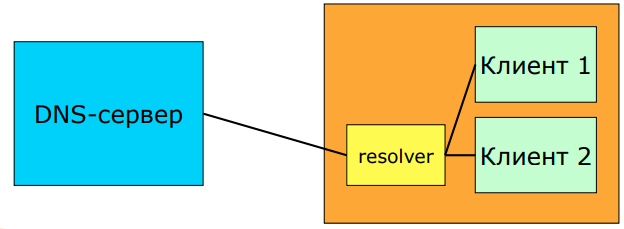
\includegraphics[width=15cm]{images/05/02}
\end{figure}

\Subsubsection{Организация DNS и прямой поиск}

Всё дерево имен поделено на участки ответственности~--- зоны.

Для каждой зоны существует свой сервер DNS, отвечающий за зону. Сервер, отвечающий за зону~--- авторитетный сервер.

Для каждой зоны должно быть несколько авторитетных серверов: один~--- первичный (содержит исходную информацию о зоне), несколько вторичных (содержат копию информации о зоне и периодически обновляют информацию).

Все сервера хранят информацию о зоне, обслуживают запросы об этой зоне, перенаправляют запросыо  других зонах вышестоящим или подчиненным серверам. Существенная часть серверов (но не все!) занимается кэшированием информации о других зонах.

Первичные серверы копирую зонную информацию вторичным и подифицируют первичную информацию.

Вторичные серверы периодически опрашивают первичных.

Типы DNS серверов по способу ответа на запрос:
\begin{itemize}
    \item Рекурсивные серверы
    \begin{itemize}
        \item Самостоятельно выполняют весь поиск (если они не ответственны за эту зону)
        \item Кэшируют полученную информацию
    \end{itemize}
    \item Нерекурсивные серверы
    \begin{itemize}
        \item Указывают, где есть необходимая информация
        \item Не кэшируют информацию
    \end{itemize}
\end{itemize}

Чем ближе сервер к клиенту, тем больше вероятность, что он рекурсивный.

Все серверы первого уровня~--- нерекурсивные.

У каждого компьютера сконфигурирован DNS-сервер по умолчанию.

Пусть мы хотим обратиться к сайту spb.hse.ru.

Ресолвер смотрит, нет ли у него информации. Если нет~--- обращается к DNS-серверу по умолчанию. Тот смотрит, нет ли у него информации. Если нет, то обращается к одному из корневых серверов (их всего 13 штук и о них позже). Он нерекурсивный, поэтому возвращает нам адрес того, где нужно искать и мы сами обращаемся по тому адресу. Ну и так далее, пока не найдётся нужное имя.

Это называется процедурой прямого поиска.

{\bf Корневые серверы.}

Их 13 штук. На территории России и Африки нет ни одного.

К корневому серверу очень большой трафик.

Например, в Москве сделали зеркало корневого сервера. Провайдеры перехватывают запросы к корневым серверам и перепосылают его на зеркало, экономя трафик.

Кстати, в корпоративной сети РЖД несколько миллионов компьютеров, они подняли свой DNS со своим корневым доменом.

Вся база данныз DNS состоит из ресурсных записей (RR).

Дальнейший рассказ будет использовать терминологию системы bind (Berkeley Internet Name Domain)~--- это ведущий name-сервер в мире и его терминология используется повсеместно.

Каждая запись хранит определённый тип информации и содержит следующие поля:
\begin{itemize}
    \item Имя (необязательное). В случае отсутствия используется предыдущее
    \item Класс записи (для Интернета - IN)
    \item Тип записи
    \item Время актуальности (необязательное). В случае отсутствия используется значение по умолчанию. Сколько данную запись можно держать в кэше
    \item Параметры записи (зависят от типа)
\end{itemize}

Существует несколько типов записей.

{\bf Адресная запись.}

Подавлющее число записей имеют этот тип.

Обозначается <<A>>

Параметры:
\begin{itemize}
    \item Доменное имя узла
    \item Соответствующий адрес
\end{itemize}
Формат bind:
\begin{itemize}
    \item name IN A address
\end{itemize}
Пример: {\tt school IN A 195.19.212.16}

Обратим внимание, что здесь нет точки. Это относительный адрес. Это означает, что подразумевается домен по умолчанию для этого DNS-сервера

{\bf Запись о сервере имён.}

Обозначается <<NS>>

Позволяет задать вторичный сервер имём

Параметры:
\begin{itemize}
    \item Имя домена
    \item Адрес сервера имён
\end{itemize}
Формат bind:
\begin{itemize}
    \item domain IN NS address
\end{itemize}
Пример: {\tt school.server.ru. IN NS 195.19.212.13}

Для домена {\tt school.server.ru.} указали, что у него есть вторичный DNS-сервер по такому-то адресу.

Как минимум одна такая запись должна быть в домене.

 {\bf Главная ресурсная запись.}

 Обозначается <<SOA>> (start of authority)

 Описывает основные параметры зоны.

 Параметры:
 \begin{itemize}
    \item Имя домена
    \item Имя первичного DNS-сервера (вторичный задаётся через запись NS)
    \item Почтовый адрес администратора
    \item Серийный номер зоны (Serial)~--- уникальный идентификатор, который увеличивается по мере изменения зоны. Является ключом для вторичного сервера. Если вторичный сервер видит, что идентификатор изменился, то он понимает, что зона изменилась и зону нужно скопировать 
    \item Период обновления (Refresh)~--- как часто вторичный сервер должен обращаться за изменением информации
    \item Время валидности данных зоны (Expire)~--- как долго вторичный сервер будет отвечать на доменные запросы, если первичный не отвечает
    \item Период повторных попыток (Retry)~--- период повторных попыток вторичного обратиться к первичному, если первичный не ответил.
    \item Значение по умолчанию (DefaultTTL)~--- дефолтное время кэширования для всех записей в зоне
\end{itemize}

Должна быть одна на зону.

Формат bind: {\tt domain IN SOA ns e-mail (Serial Refresh Retry Expire DefaultTTL)}

Пример: {\tt school.server.ru. IN SOA ns.school.server.ru. admin.school.server.ru. (2008121801 3600 900 2592000 900)}

Домен {\tt school.server.ru.}. У него есть первичный сервер. Адрес почты администратора~--- {\tt admin@school.rerver.ru} (собака зарезервирована).

Запись скорее всего от 18 декабря 2008 года, номер изменения 01. Так администраторы часто ведут зону.

Refresh~--- раз в час. Retry~--- 15 минут. Expire~--- месяц. DefaultTTL~--- 15 минут.

При запросе копии зоны вторичным сервером используется тип передачи AXFR (о том, что это такое~--- позже).

Этих трёх записей достаточно для функционирования DNS. Но у DNS есть и дополнительные функции.

{\bf Запись о сервере электронной почты}

Обозначается <<MX>>

Параметры:
 \begin{itemize}
    \item Имя почтового домена
    \item Имя почтового сервера
    \item Приоритет
\end{itemize}

Формат bind: {\tt Mail-domain IN MX priority address}

Пример: \\
{\tt office IN MX 10 mail.school.server.ru.}\\
{\tt office IN MX 20 mail.yandex.ru.}

Если кто-то послал почту по адресу {\tt xxx@office.ИМЯНАШЕГОДОМЕНА}. Посылаем сначала на первый, а если он вдруг не отвечает, то на второй.

{\bf Запись о псевдониме.}

Обозначается <<CNAME>>

Параметры:
\begin{itemize}
    \item Доменное имя узла (псевдоним)
    \item Реальное (каноническое имя)
\end{itemize}

Формат bind: {\tt сname IN CNAME name}

Пример: {\tt www IN CNAME node.school.server.ru.}

Если кто-то обратится по адресу {\tt www.ИМЯНАШЕГОДОМЕНА}, на самом деле это превратится в адрес {\tt node.sschool.server.ru.}

Псевдонимы запрещены при маршрутизации почты.

{\bf Запись о сервисе.}

Обозначается <<SRV>>.

Формат bind: {\tt \_Service.\_Proto.Name IN SRV Priority Weight Port Target}

Параметры:
\begin{itemize}
    \item Service~--- имя сервиса
    \item Proto~--- имя протокола
    \item Priority~--- приоритет
    \item Weight~--- вес (для балансировки нагрузки). Доля запросов, которые пойдут на этот сервис
    \item Target~--- имя узла, на котором находится сервис
\end{itemize}

Пример:\\
{\tt \_xmpp-server.\_tcp.example.ru. 3600 IN SRV 20 0 5269 jabber1.ru.}\\
{\tt \_xmpp-client.\_tcp.example.ru. 3600 IN SRV 20 90 5222 jabber1.ru.}\\
{\tt \_xmpp-client.\_tcp.example.ru. 3600 IN SRV 20 10 5222 jabber2.ru.}

Здесь показан способ балансировки нагрузки нагрузки. 90\% запросов будут идти к первому клиенту, а 10\% ко второму.

Через запись SRV можно полностью повторить запись MX.

{\bf Другие ресурсные записи}
\begin{itemize}
    \item WKS~--- анонсирование сервисов~--- сообщает, какие сервисы запущены на данном узле. Не используется, так как использовалась хакерами
    \item HINFO~--- информация об узле. Опять мечта для хакера.
    \item RP~--- Responsable Person~--- почтовый адрес ответственного за узел, но эту запись никто не заполнял и она не используется.
    \item TXT~--- текстовая запись. Раньше: <<Любая дополнительная текстовая информация, которую вы хотите сообщит миру о своём узле>>. Сейчас: <<Запись, куда можно поместить любую информацию об узле. В том числе, автоматически обрабатываемую.>>. Используется. Могут размешаться, например, открытые ключи.
    \item ...
\end{itemize}

\Subsubsection{Обратный поиск}

Хотим по IP-адресу узнать доменное имя. 

Цель следующая: убедиться, что адрес валидный и на него зарегистрировано доменное имя. Используется в целях безопасности.

Используются механизмы прямого поиска. Для этого введён специальный домен: {\tt in-addr.arpa.}. Имена состоят из октетов IP-адресов.

При запросу имени для адреса X.Y.Z.T строится запрос для
имени: {\tt T.Z.Y.X.in-addr.arpa} и такой запрос обслуживается как прямой.

Пример:\\
Адрес {\tt 195.19.212.97}\\
Доменное имя: {\tt 97.212.19.195.in-addr.arpa.}

Введена ресурсная запись PTR

Используется для преобразования имён из домена in-addr.arpa. в доменное имя.

Параметры:
\begin{itemize}
    \item Имя узла в домене in-addr.arpa.
    \item Доменное имя узла
\end{itemize}

Формат bind: {\tt in-addr-name IN PTR name}

Примеры:\\
{\tt 11.12.19.195.in-addr.arpa. IN PTR ya.ru}\\
{\tt 16 IN PTR office.school.server.ru}

\Subsection{Система bind}

Организация базы данных DNS.
\begin{itemize}
    \item Главный файл конфигурации {\tt /etc/named.conf}
    \item Файл прямого преобразования {\tt /var/named/ftk.hosts}
    \item Файл обратного преобразования {\tt /var/named/ftk.rev}
    \item Файл кэша корневых серверов {\tt /var/named/named.ca}
    \item Файл обратного преобразования локальной зоны {\tt /var/named/local.rev}~--- чтобы {\tt 127.0.0.1} преобразовывалось в {\tt localhost}
\end{itemize}

\Subsection{Расширения DNS}

\Subsubsection{Динамические обновления}

Существуют динамические системы управления адресами (DHCP) (динамическая смена IP-шника). И те, кто ими пользуются, при получении нового IP, хотят иметь старое доменное имя.

Идея: авторизованный клиент (например, DHCP сервер) посылает серверу DNS запрос на изменение ресурсной записи. Если сервер не первичный, запрос пересылается наверх, пока запрос не дойдёт до первичного. Когда запрос дошёл до первичного сервера, тот заносит информацию в свою БД, инкрементирует номер зоны, а вторичные серверы потом это подхватят.

\Subsubsection{Нотификация}

Асинхронное информирование об изменении информации~--- технология DNS NOTIFY.

Первичный сервер посылает сообщение <<У меня есть обновление!>> всем известным ему вторичным, вторичные посылают всем другим вторичным (редко бывает, что первичный не знает обо всех вторичных, но такое встречается). Каждое сообщение от первичного подтверждается. Вторичные осуществляют запрос зоны как при периодическом обновлении.

\Subsubsection{Инкрементальная передача зон}

При частом обновлении информации слишком много трансферов зон. Поэтому придумали пересылать не всю зону, а только то, что изменилось.

Вторичный посылает свой серийный номер зоны, первичный считает дельту и отправляет её.

Тип запроса~--- IXFR.

\Subsection{Ещё пару слов о DNS}

\Subsubsection{Серверы-ретрансляторы}

Их используют для сокращения внешнего трафика.

Пусть у нас много трафика. Выделим сервер-ретранслятор. Он не будет обслуживать никакую зону, а только обслуживает запросы наших серверов (принимает запросы от них и отсылает в интернет). И его кэш разделяется нашими серверами. Здорово экономит трафик.

Они кэшируют информацию всех запросов.

Должны конфигурироваться как ретрансляторы.

\Subsubsection{Утилиты конфигурирования}

\begin{itemize}
    \item nslookup
    \item dig
    \item host
\end{itemize}

\Subsubsection{Реализация DNS}

Для клиентских запросов и ответов используется UDP

Для зонных пересылок и клиентских запросов большого размера~--- TCP

И в UDP и в TCP порт 53

В настоящее время часто используется DNS с шифрованием.

\Subsubsection{Сосуществование различных систем именования}

В Windows сначала смотрим в Hosts, а уже потом в DNS (хакеры использовали это, подменяя Hosts).

В Unix приоритезация указывается в {\tt /etc/host.conf}

\Subsubsection{Регистрация доменных имён}

Есть море разных организаций. Например, в США это InterNIC, а в России RIPN

В домене ru управлением и поддержкой занимается RocНИИРОС (\url{ripn.net})

Они же поддерживают сервер whois~--- он позволяет сказать, на кого зарегистрирован домен.

Кроме того, есть координационный центр для доменов ru и рф (\url{cctld.ru}).

{\bf Куллстори.} Сама регистрация доменов изначально велась РосНИИРОС-ом, но 21 год назад ситуация изменилась. Раньше цена домена в домене ru была заоблочной. Это стоило 100\$ в год и 100\$ за ведение. Но Путин стал премьером, провёл совещание, на котором Артемий Лебедев прочитал огромный доклад, где заклеймил позором РосНИИРОС, мол во всех странах это стоит гораздо дешевле (ну стоит и стоит). Проблема практически сразу была решена и RIPN перестал быть регистратором доменов и стал делегировать свою функцию. Сейчас регистраторов 50 (\url{ccltd.ru/domain/reg/}).

{\bf Куллстори.} Сначала появились доменные адреса, а уже потом правительства стали думать о том, как вообще эти имена нужно регистрировать. И пока закона не было, появились киберсквотеры. Они скупали звучные доменные имена задёшево, а потом за большие деньги продавали их. Самый известный случай~--- с Microsoft. У них была Windows NT. Была Windows NT 3.5, Windows NT 4.0. А Windows NT 5.0 не было. Она стала Windows 2000. Билл Гейтс объявил это, а в течение часа умный молодой человек зарегистрировал на себя \url{windows2000.com} и перепродал Microsoft-у за 5 миллионов долларов.

{\bf Куллстори.} До гугла была поисковая система Altavista. И у неё был адрес \url{altavista.digital.com}. А адрес \url{altavista.com} прикарманила себе какая-то компания со своим простеньким поисковым движком. И они продали это имя Альтависте за большие деньги. 

Теперь есть законодательство, позволяющее обладателю товарного знака забирать такие имена.

{\bf Куллстори.} Когда в 2000-х годах мобильная связь только открывалась в России, МТС решила прийти в СПб. Для этого они решили выйти к нам под брендом <<Телеком 21>>. Киберсквотеры услышали это и в первый же день выкупили всё благозвучное с похожими именами и ждали предложений от МТС. А МТС зарегистрировались как \url{spb.mts.ru}.

\begin{figure}[h]
  \centering
  
\includegraphics[width=10cm]{images/05/03}
\end{figure}



\end{document}
